\chapter{Zeichnungen}
\newpage
\setlength{\voffset}{0cm}
\setlength{\hoffset}{0cm}
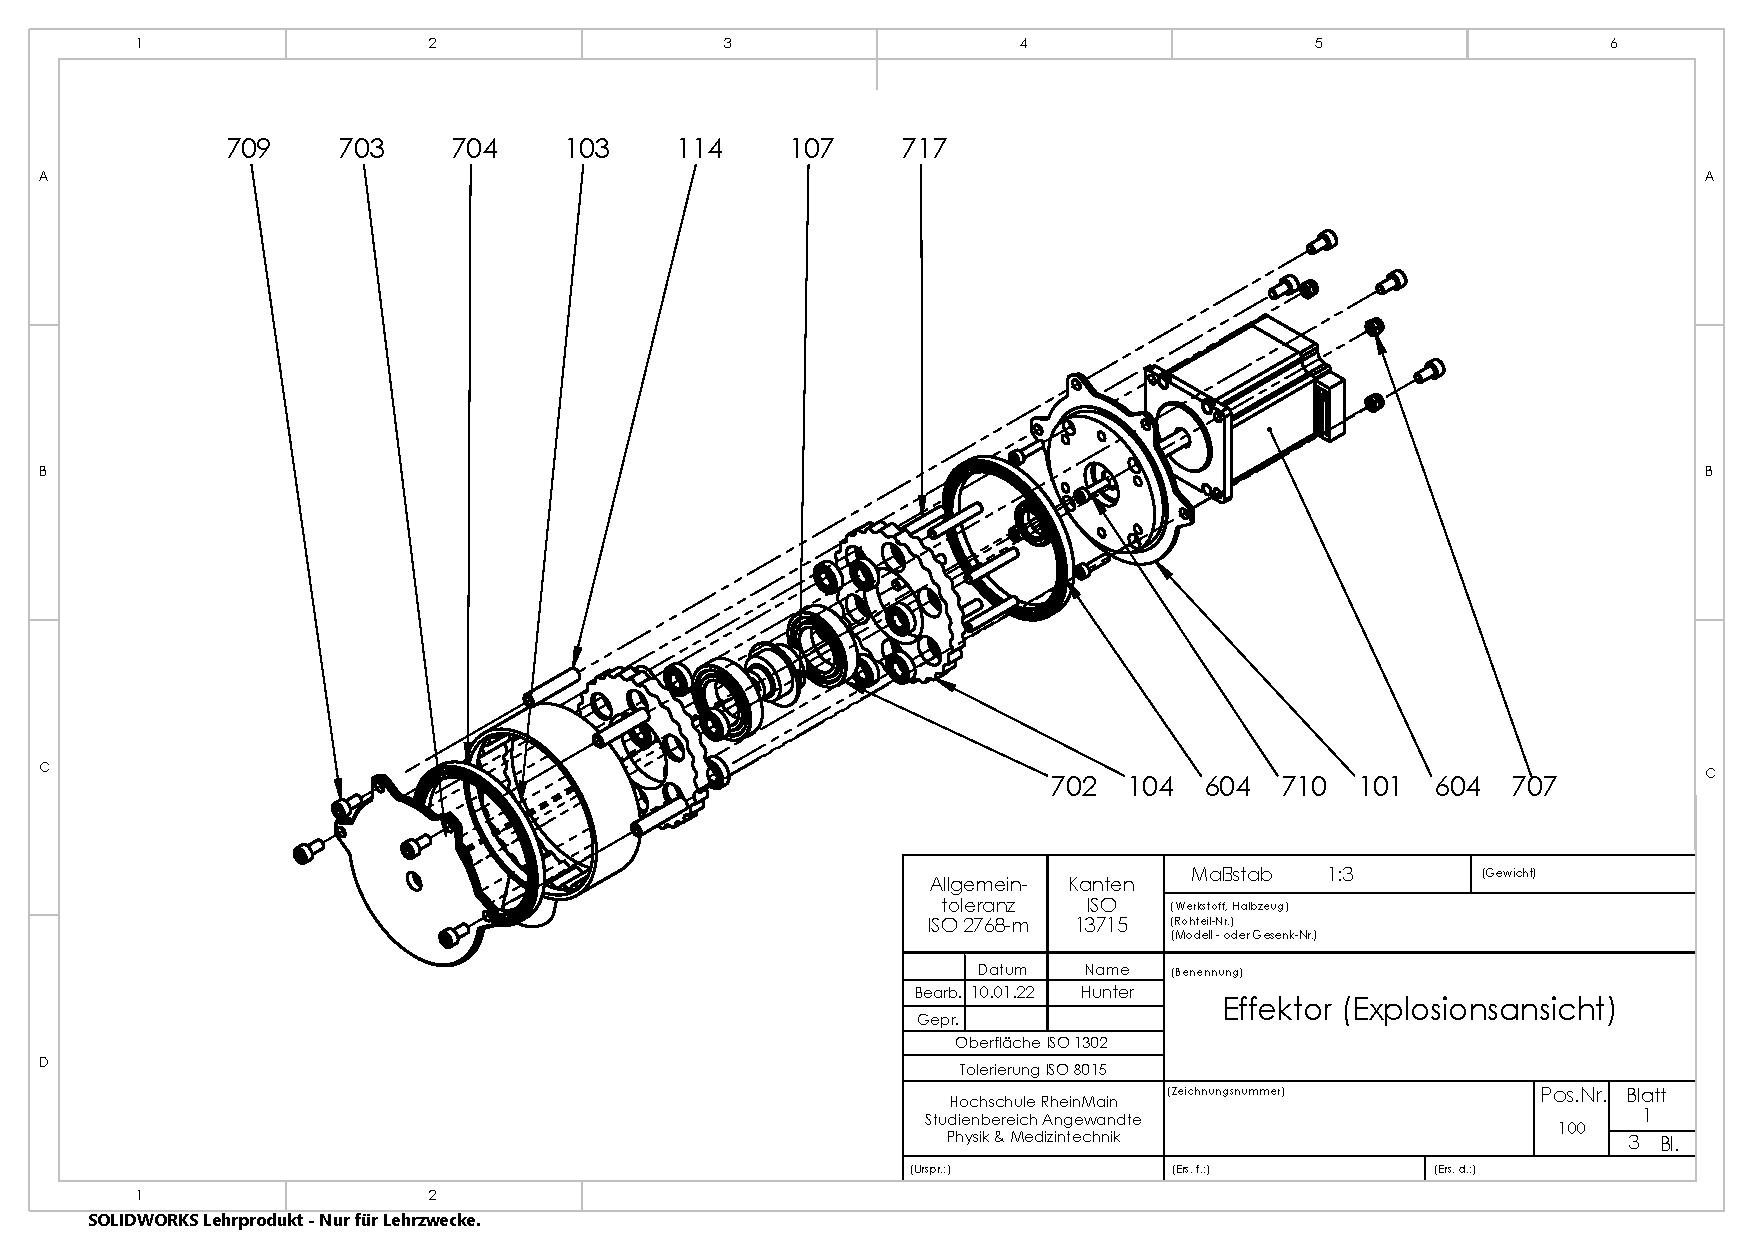
\includepdf[pages=1, angle=90, pagecommand={\thispagestyle{plain}}]{Abb/CAD/Drawings/Schulter/Effektor-assembly-drawing.pdf}
\includepdf[pages=2-3, angle=0, pagecommand={\thispagestyle{plain}}]{Abb/CAD/Drawings/Schulter/Effektor-assembly-drawing.pdf}
%
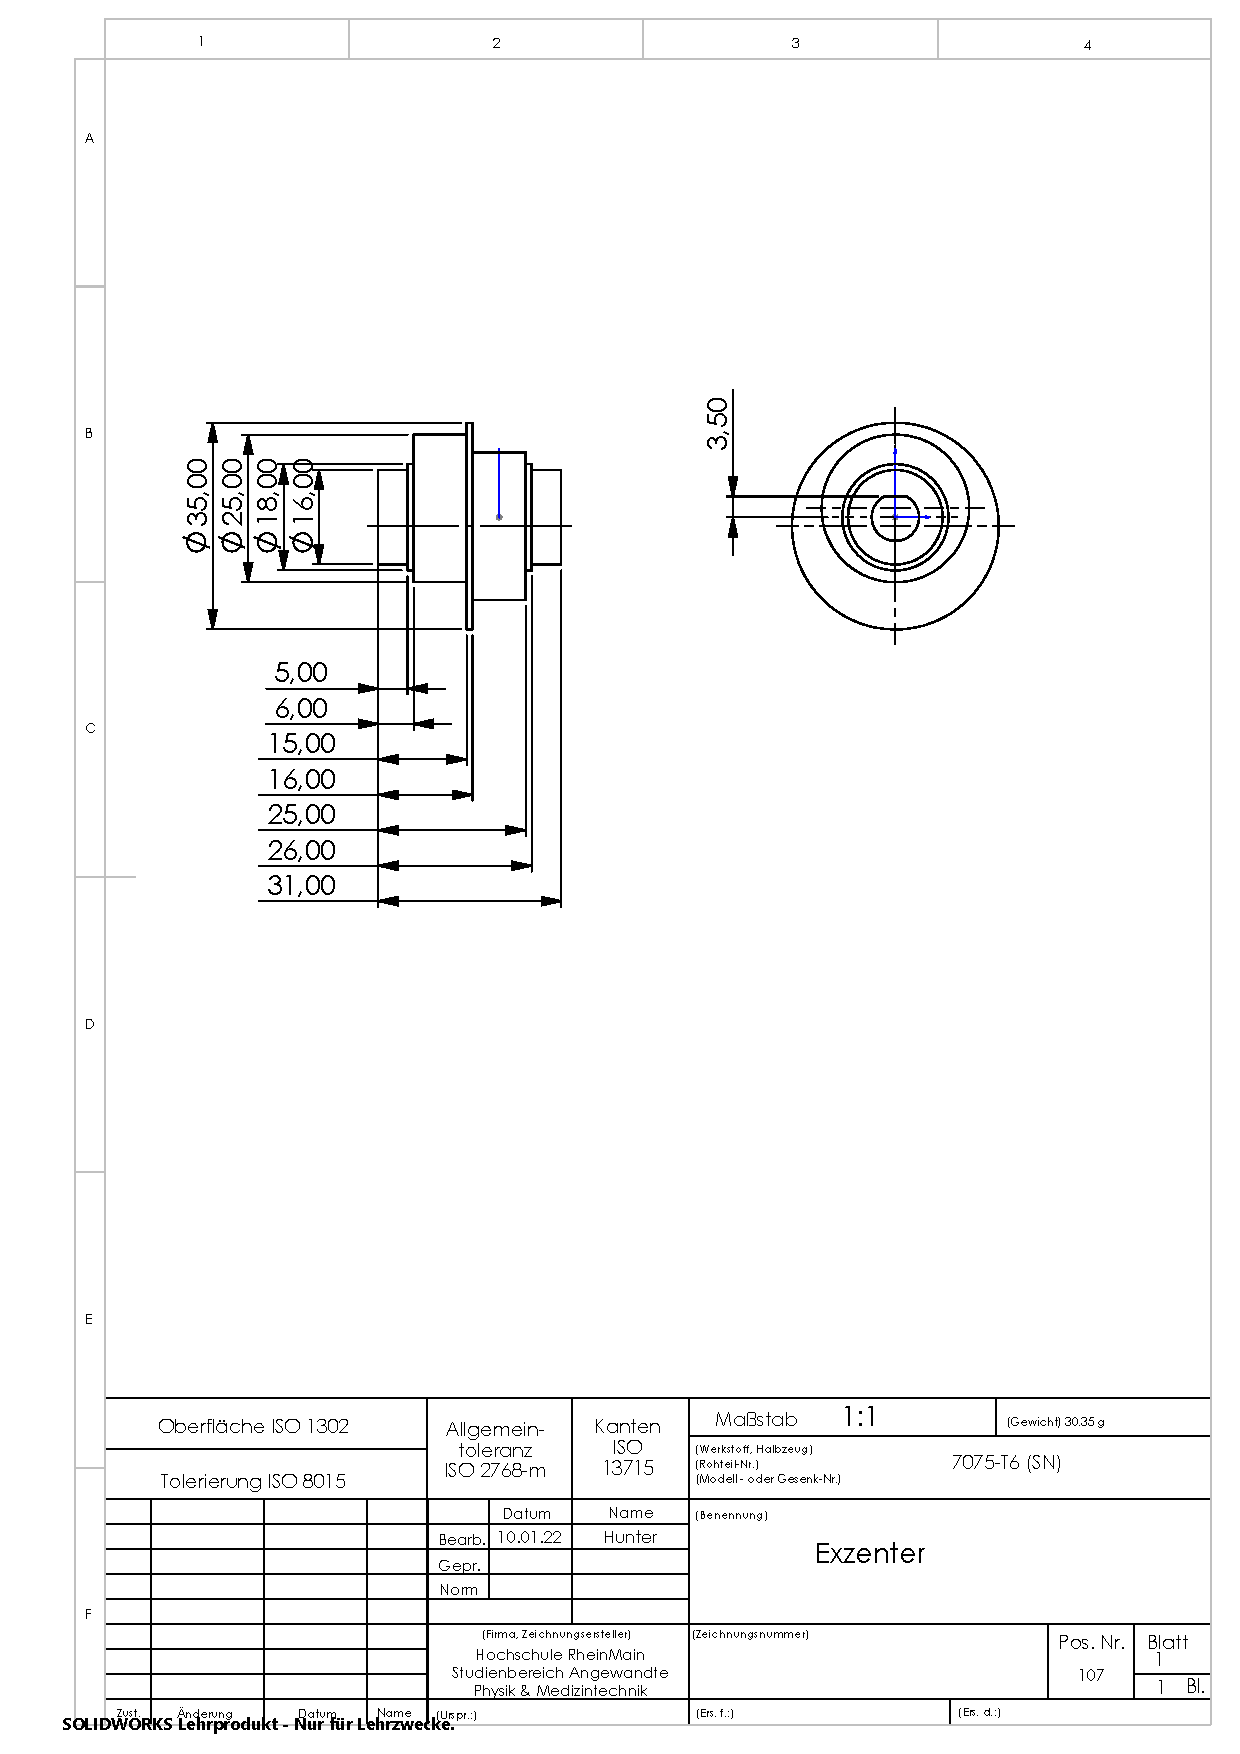
\includepdf[pages=-, angle=0, pagecommand={\thispagestyle{plain}}]{Abb/CAD/Drawings/Schulter/Exzenter.pdf}
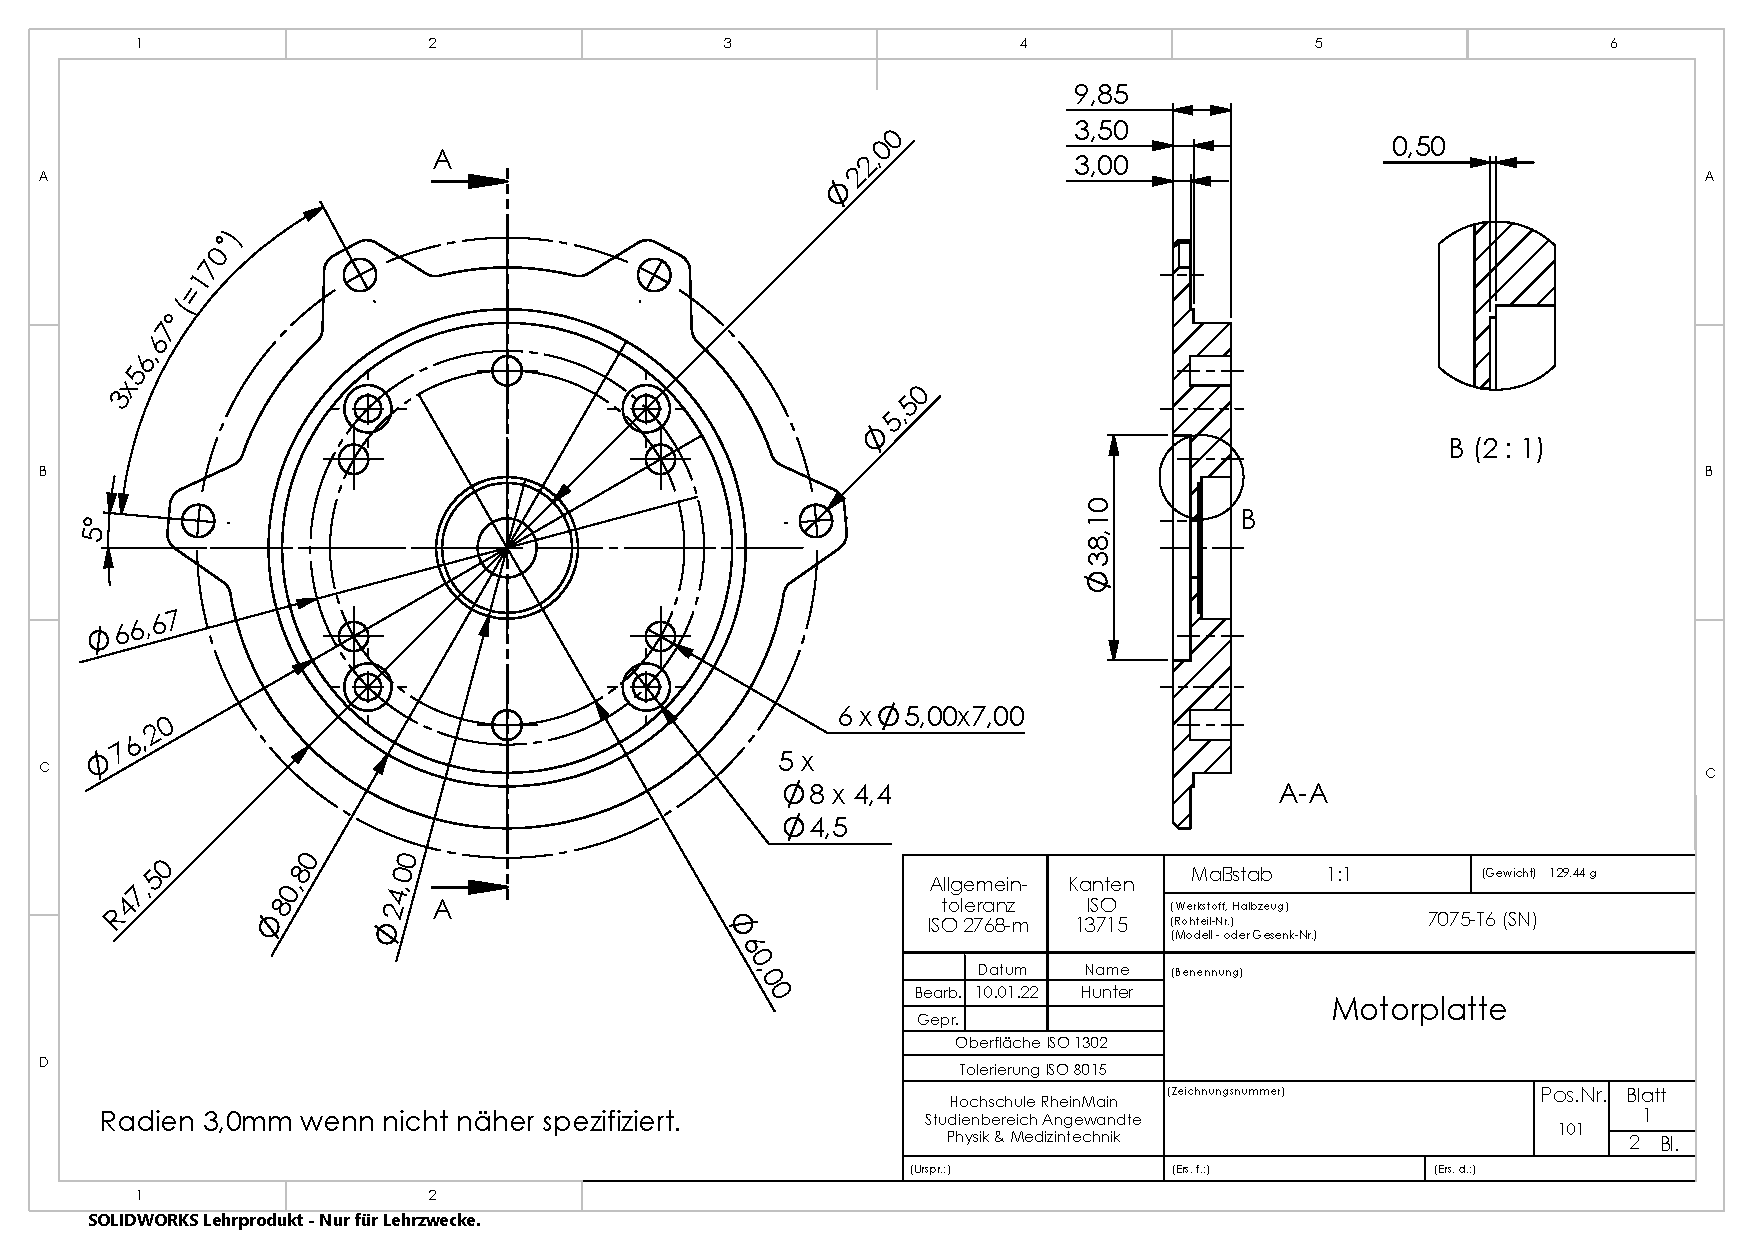
\includepdf[pages=-, angle=90, pagecommand={\thispagestyle{plain}}]{Abb/CAD/Drawings/Schulter/Motorplatte-Fixierplatte.pdf}
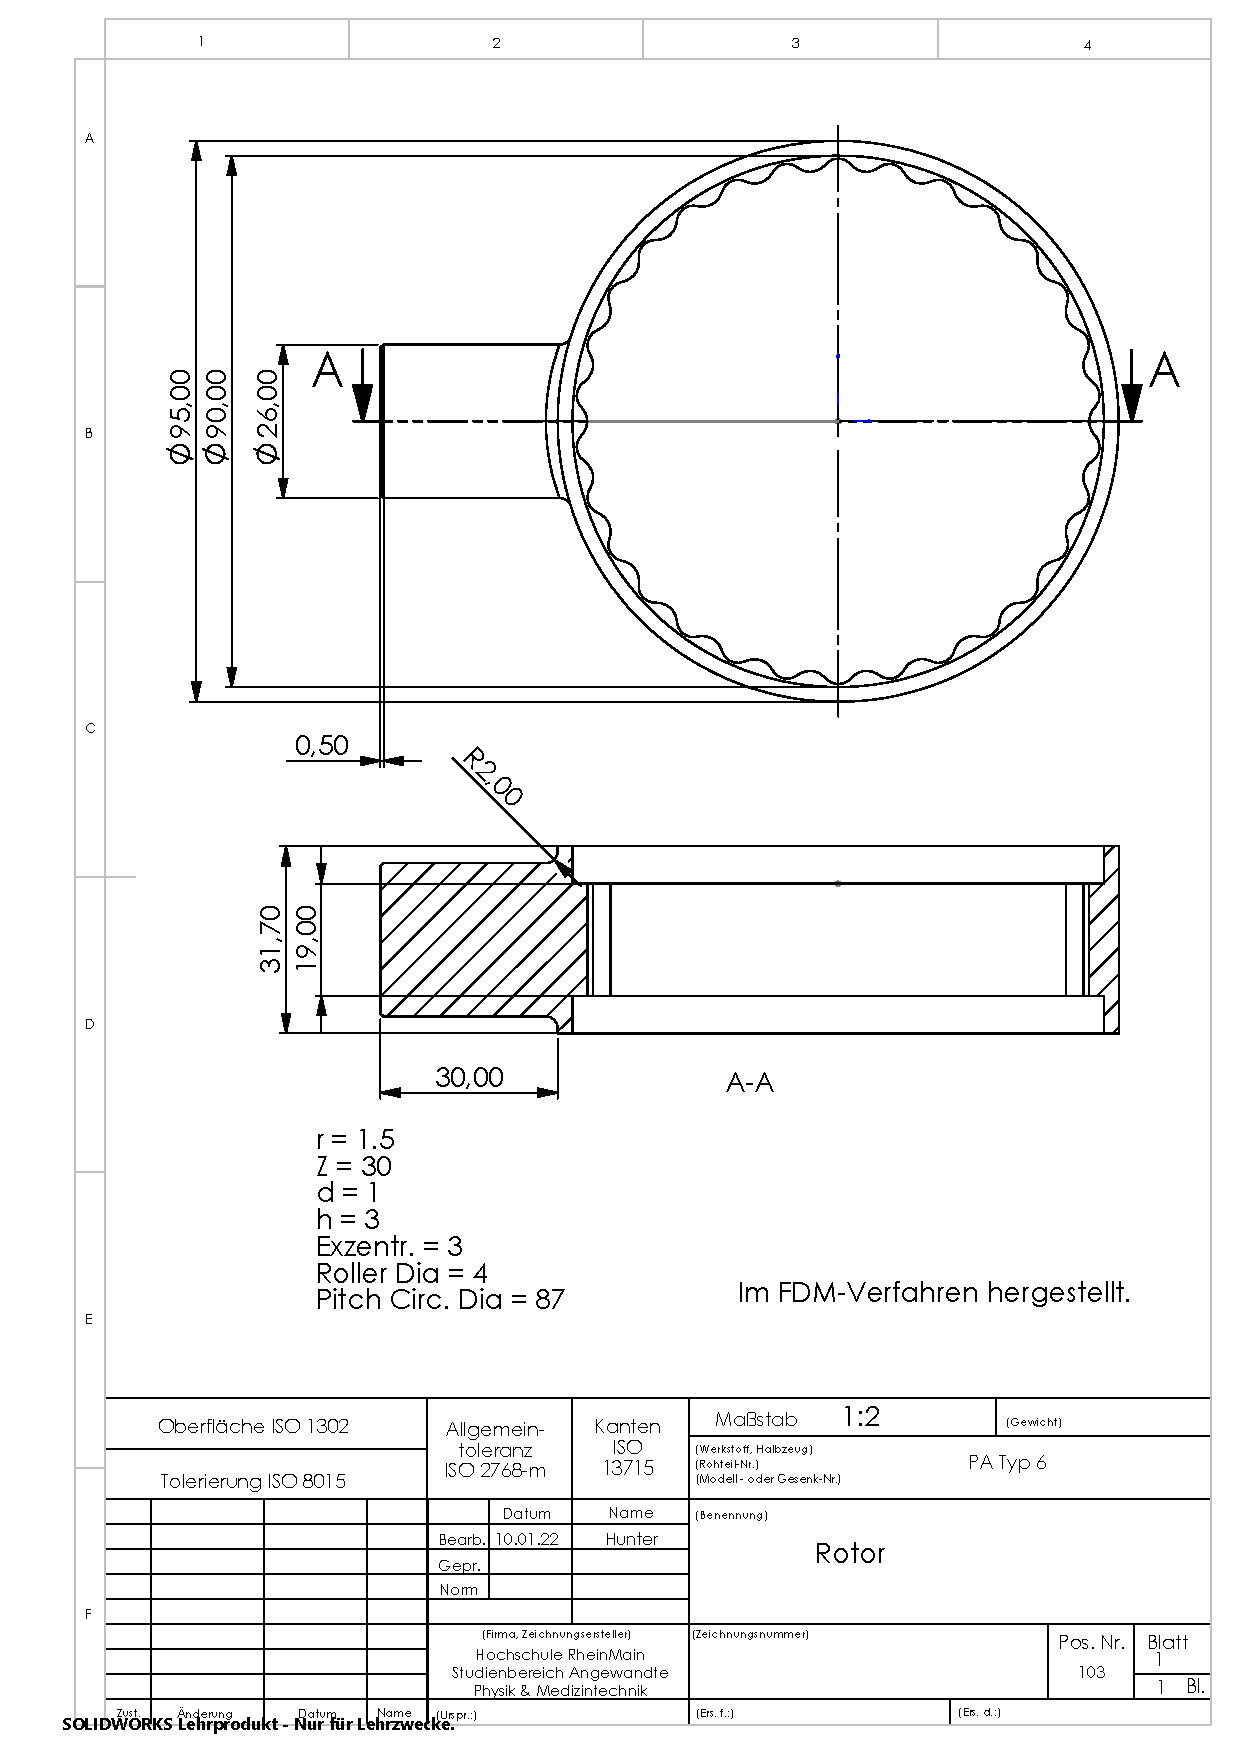
\includepdf[pages=-, angle=0, pagecommand={\thispagestyle{plain}}]{Abb/CAD/Drawings/Schulter/Rotor.pdf}
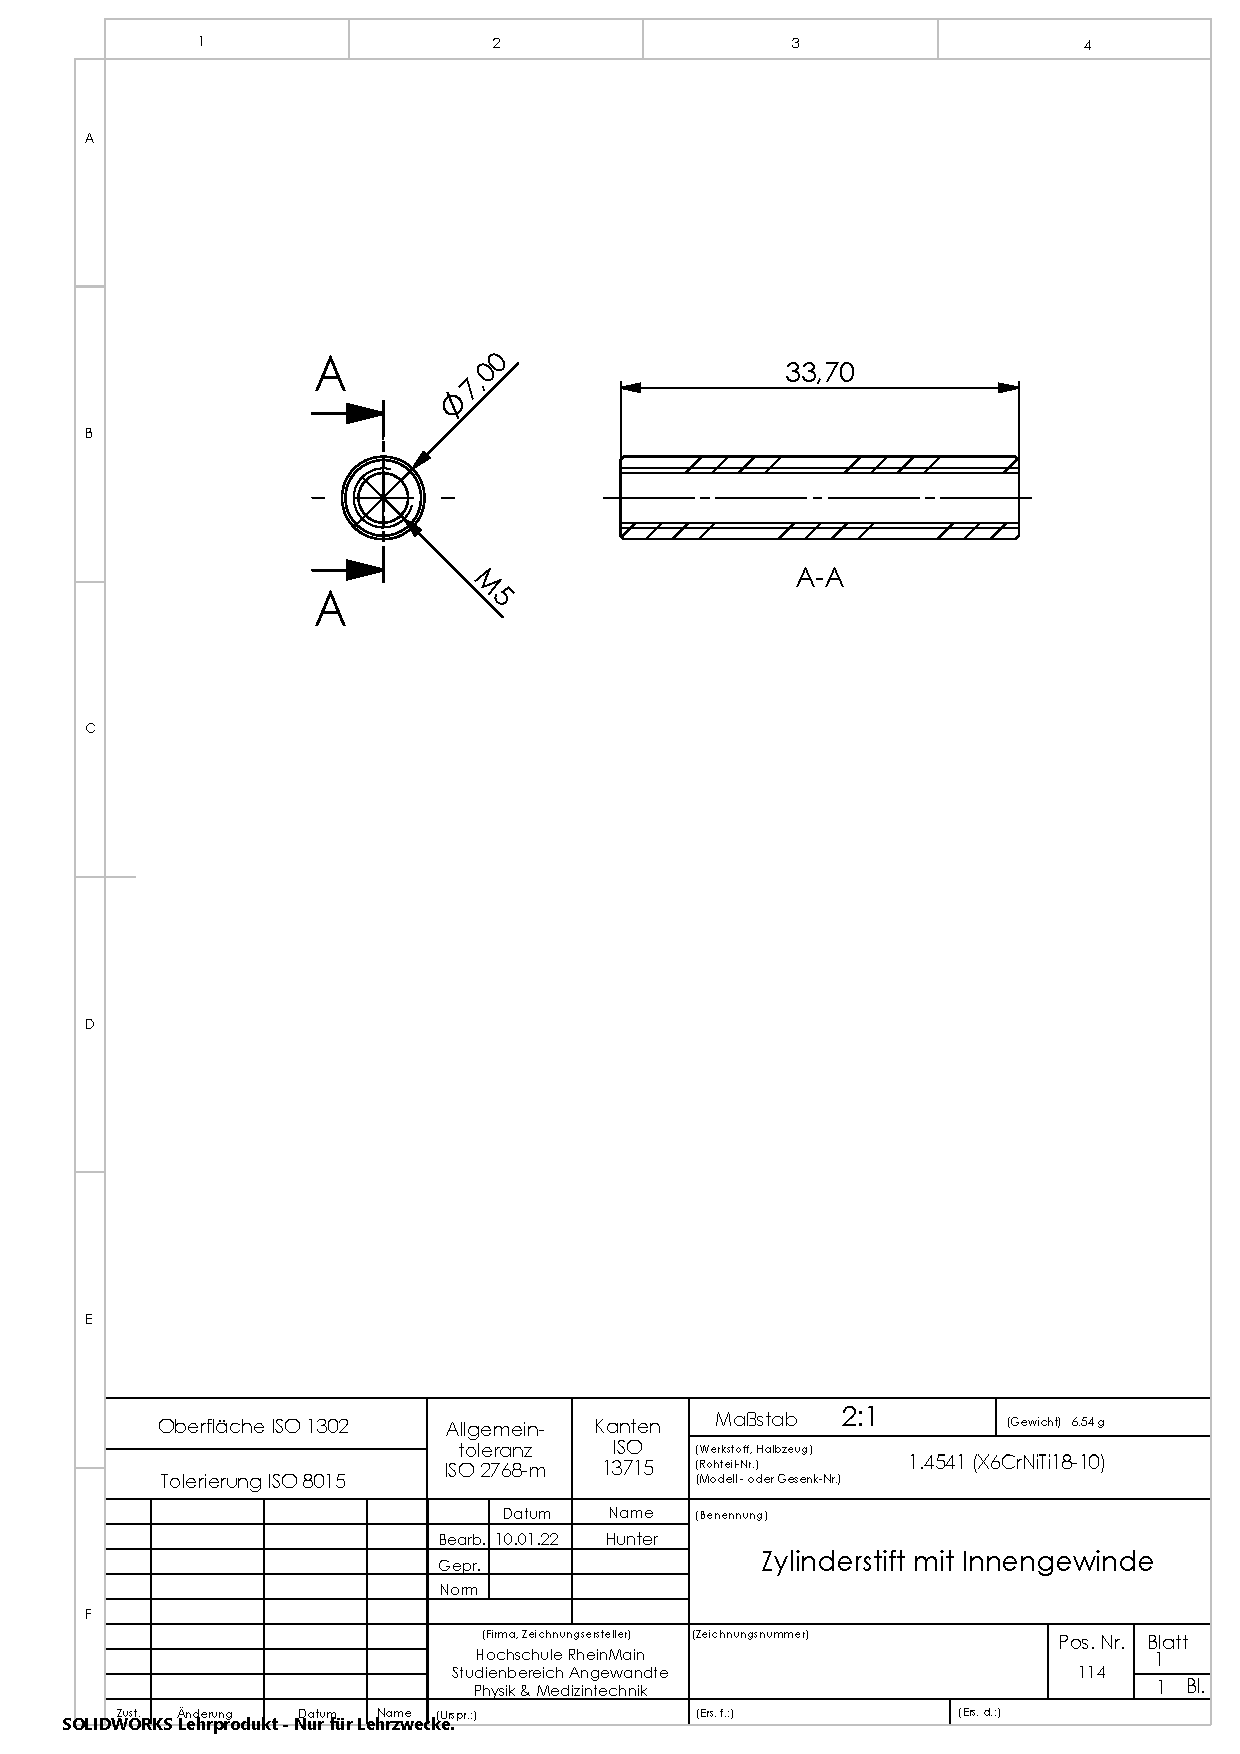
\includepdf[pages=-, angle=0, pagecommand={\thispagestyle{plain}}]{Abb/CAD/Drawings/Schulter/Zylinderstift-mit-Innengewinde.pdf}
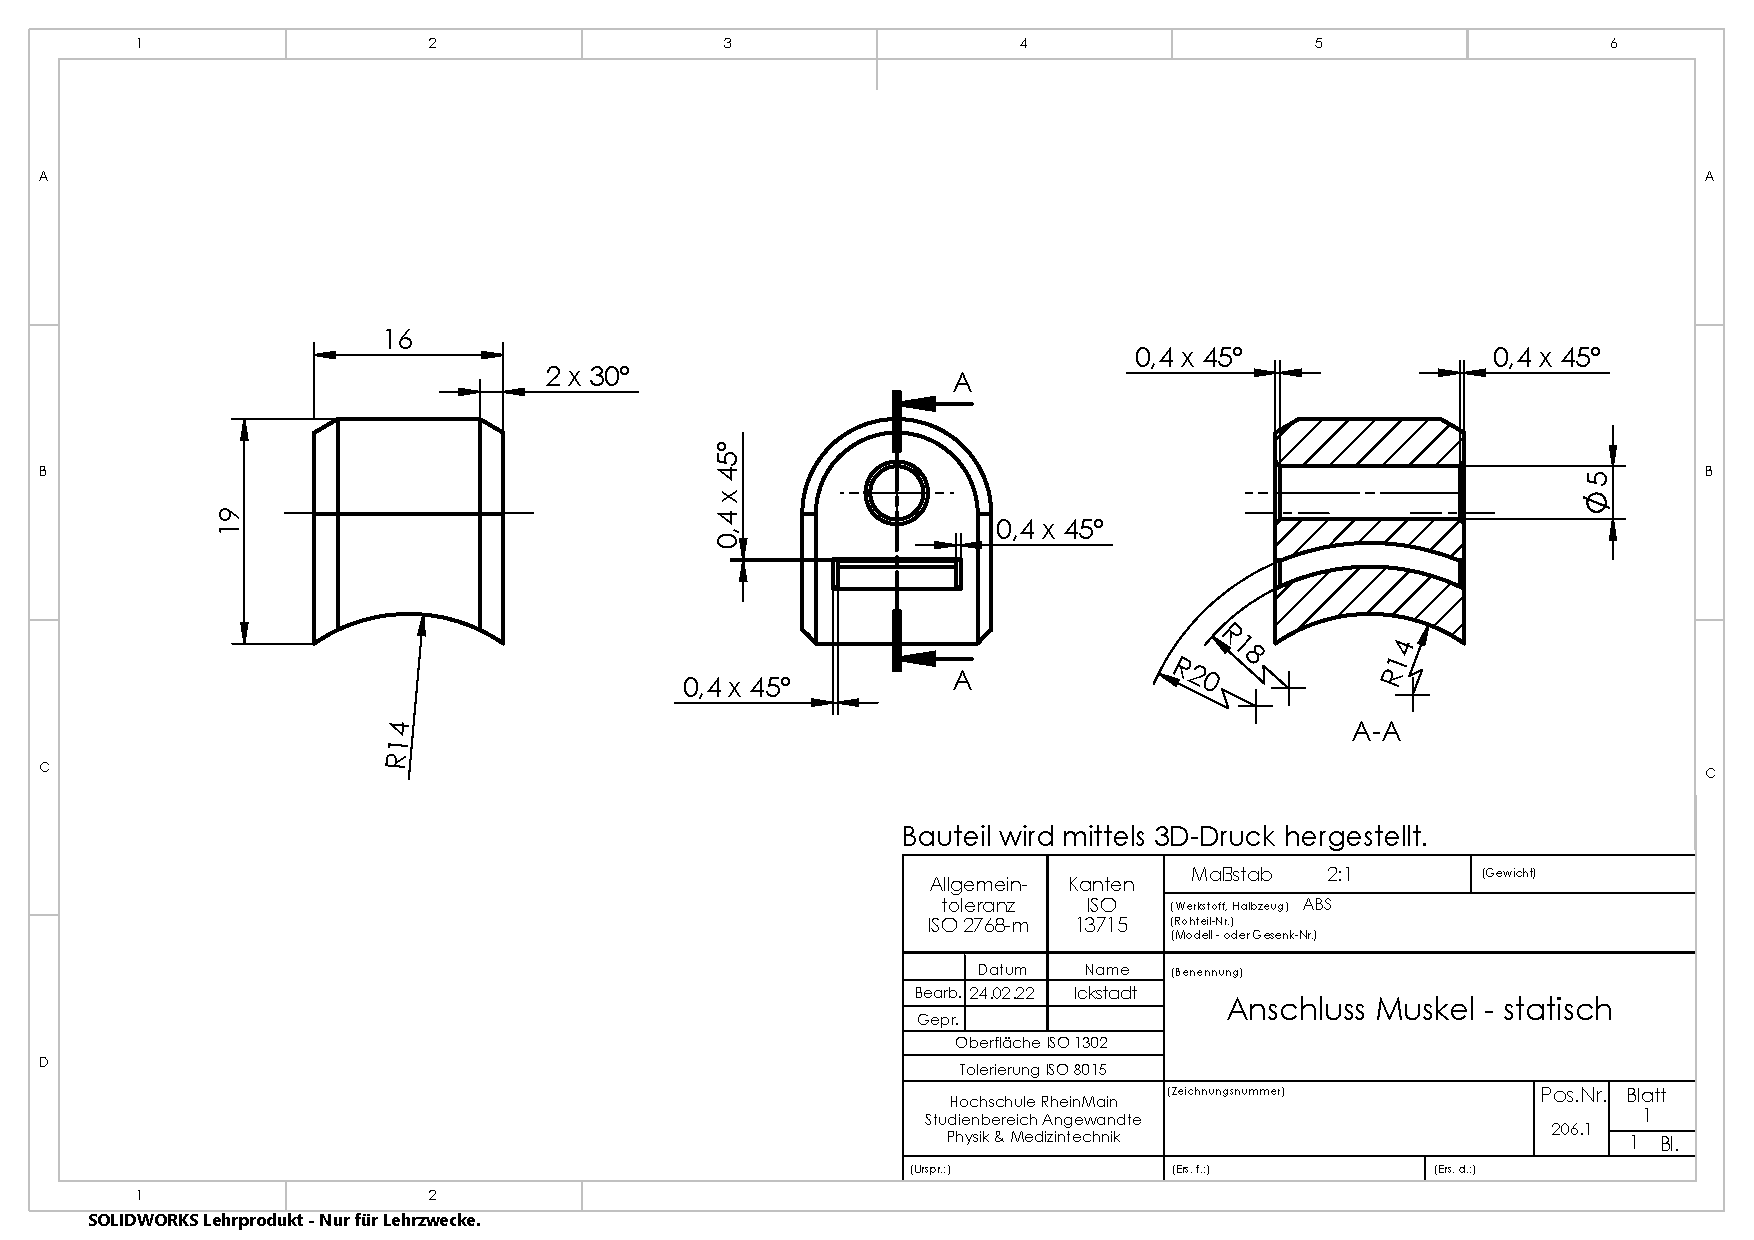
\includepdf[pages=-, angle=90, pagecommand={\thispagestyle{plain}}]{Abb/CAD/Drawings/Anschluss-Muskel-statisch.pdf}
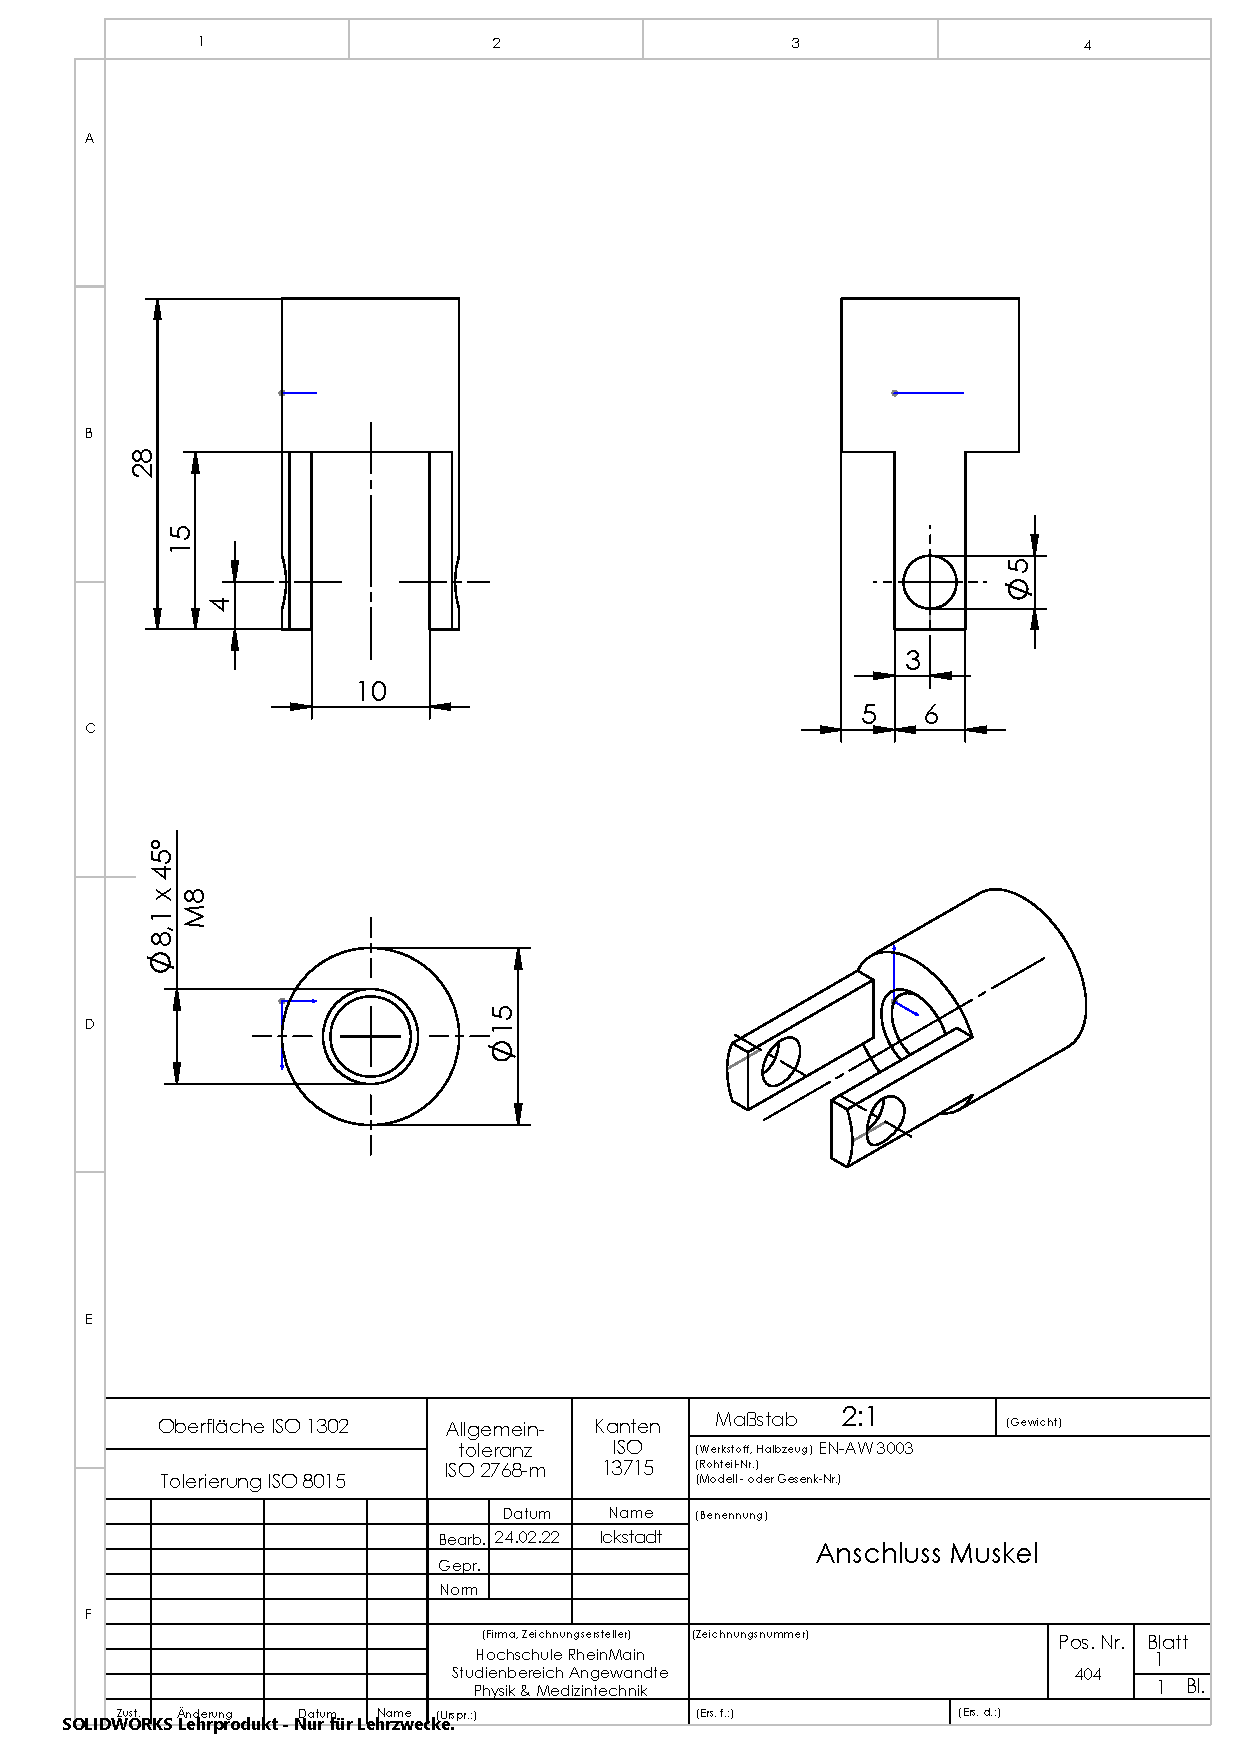
\includepdf[pages=-, angle=0, pagecommand={\thispagestyle{plain}}]{Abb/CAD/Drawings/Anschluss-Muskel.pdf}
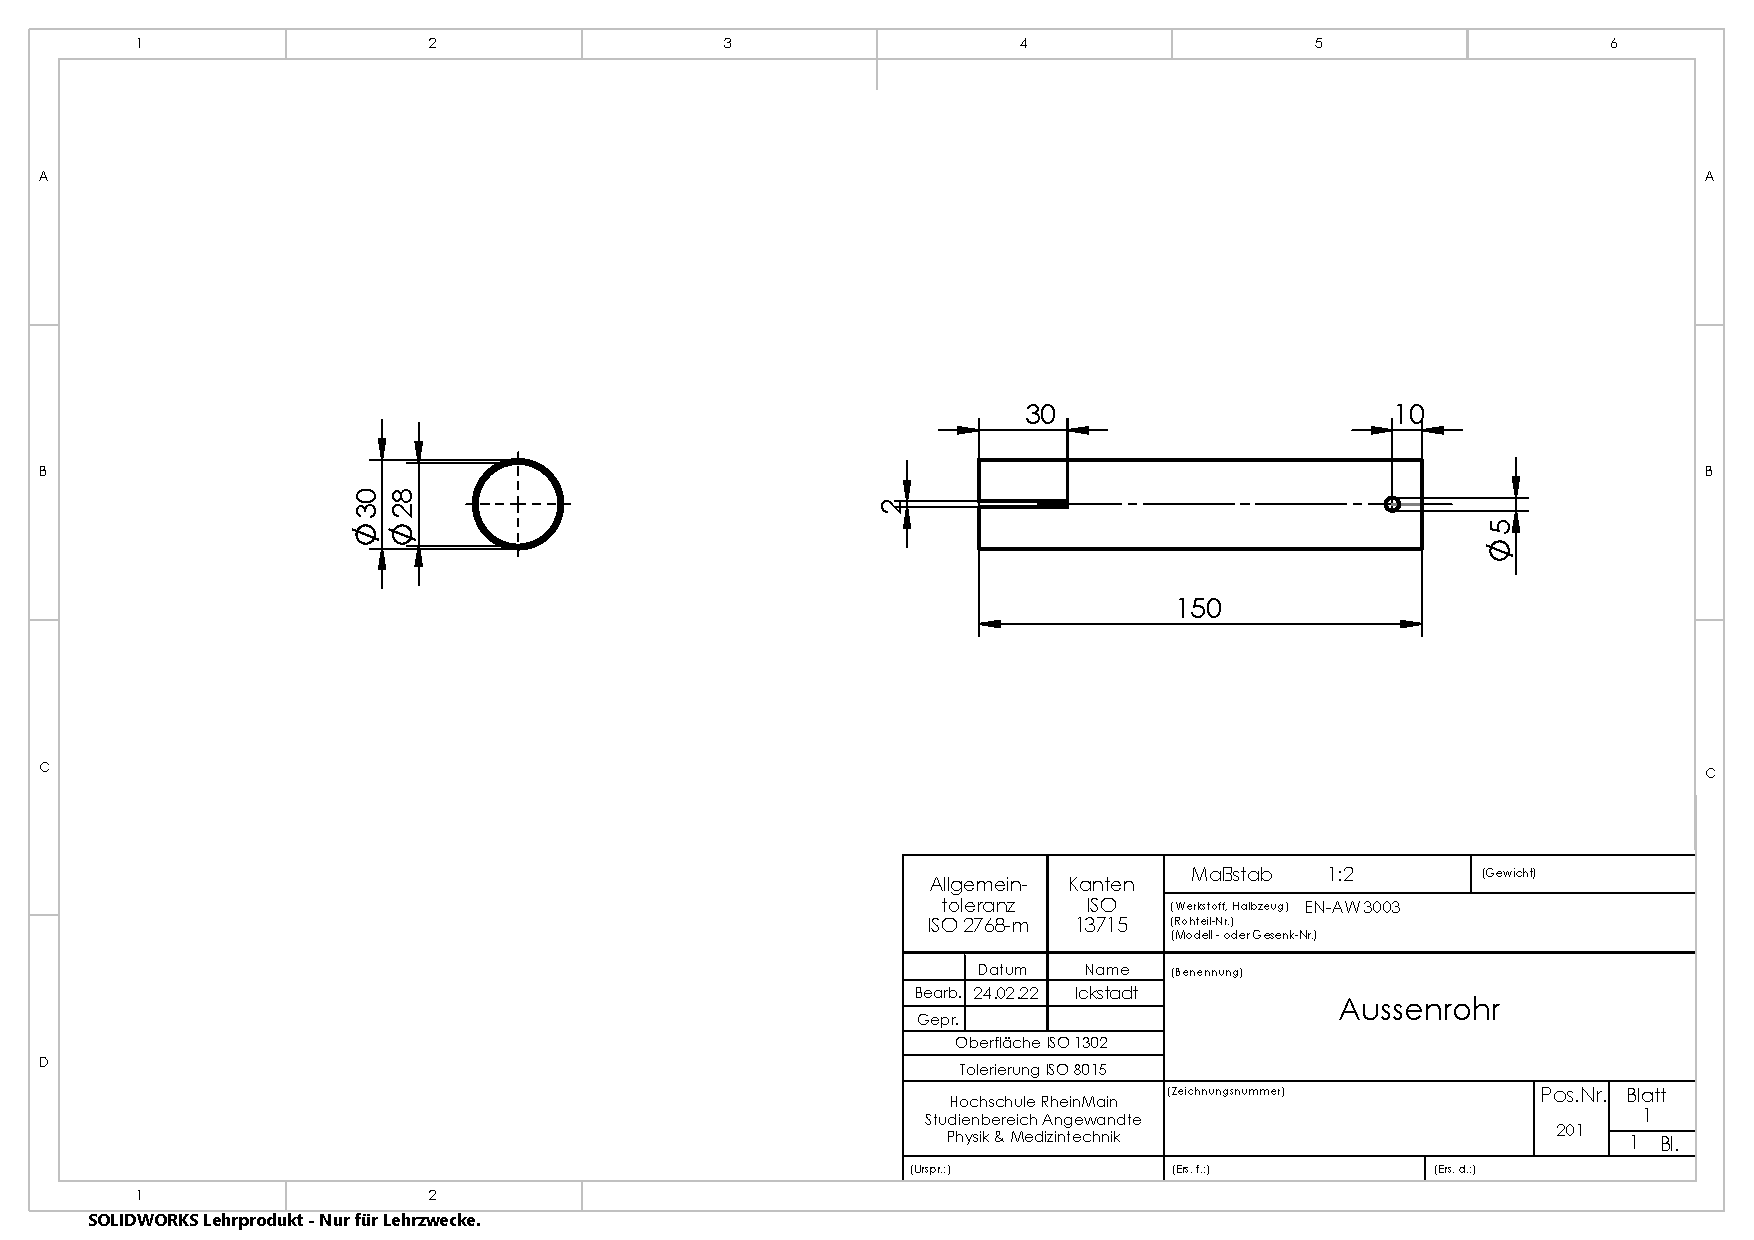
\includepdf[pages=-, angle=90, pagecommand={\thispagestyle{plain}}]{Abb/CAD/Drawings/Aussenrohr.pdf}
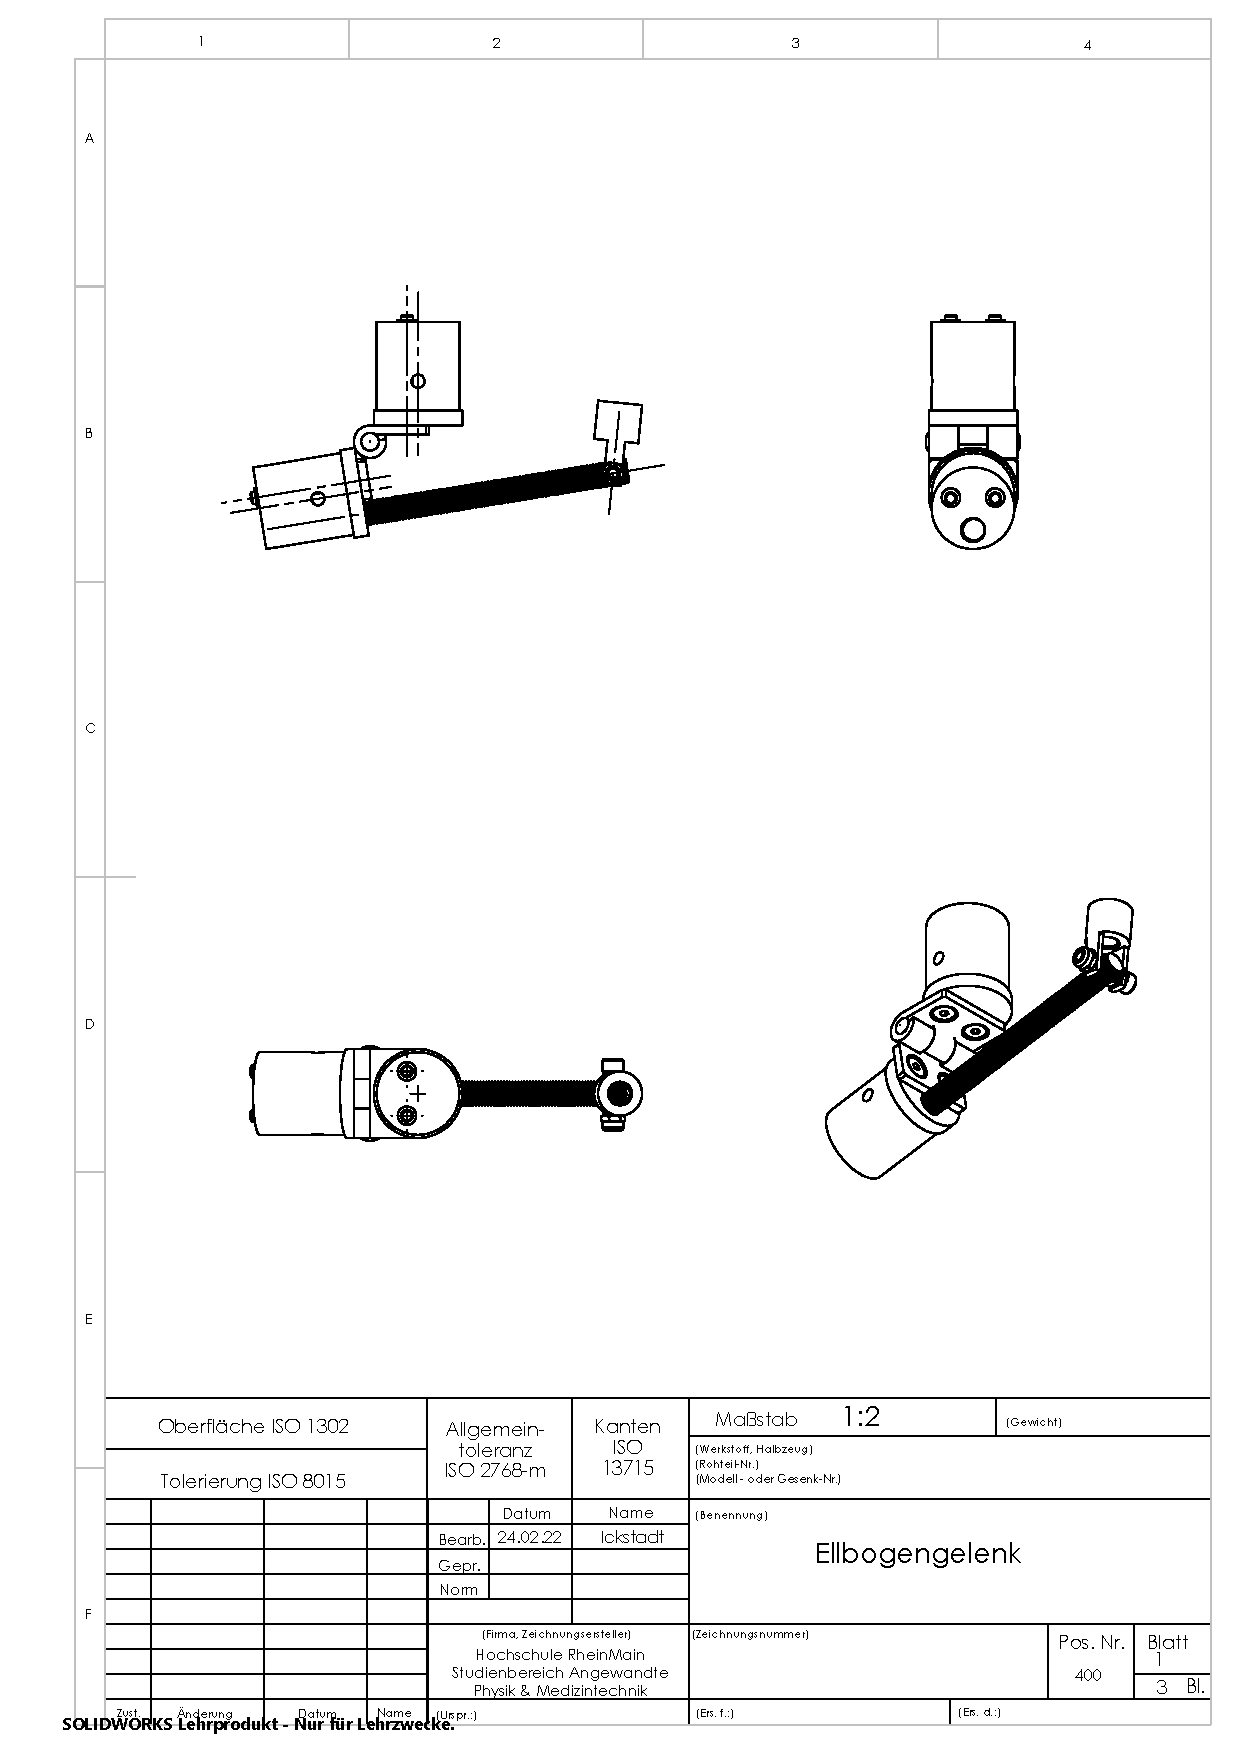
\includepdf[pages=-, angle=0, pagecommand={\thispagestyle{plain}}]{Abb/CAD/Drawings/Ellbogengelenk.pdf}
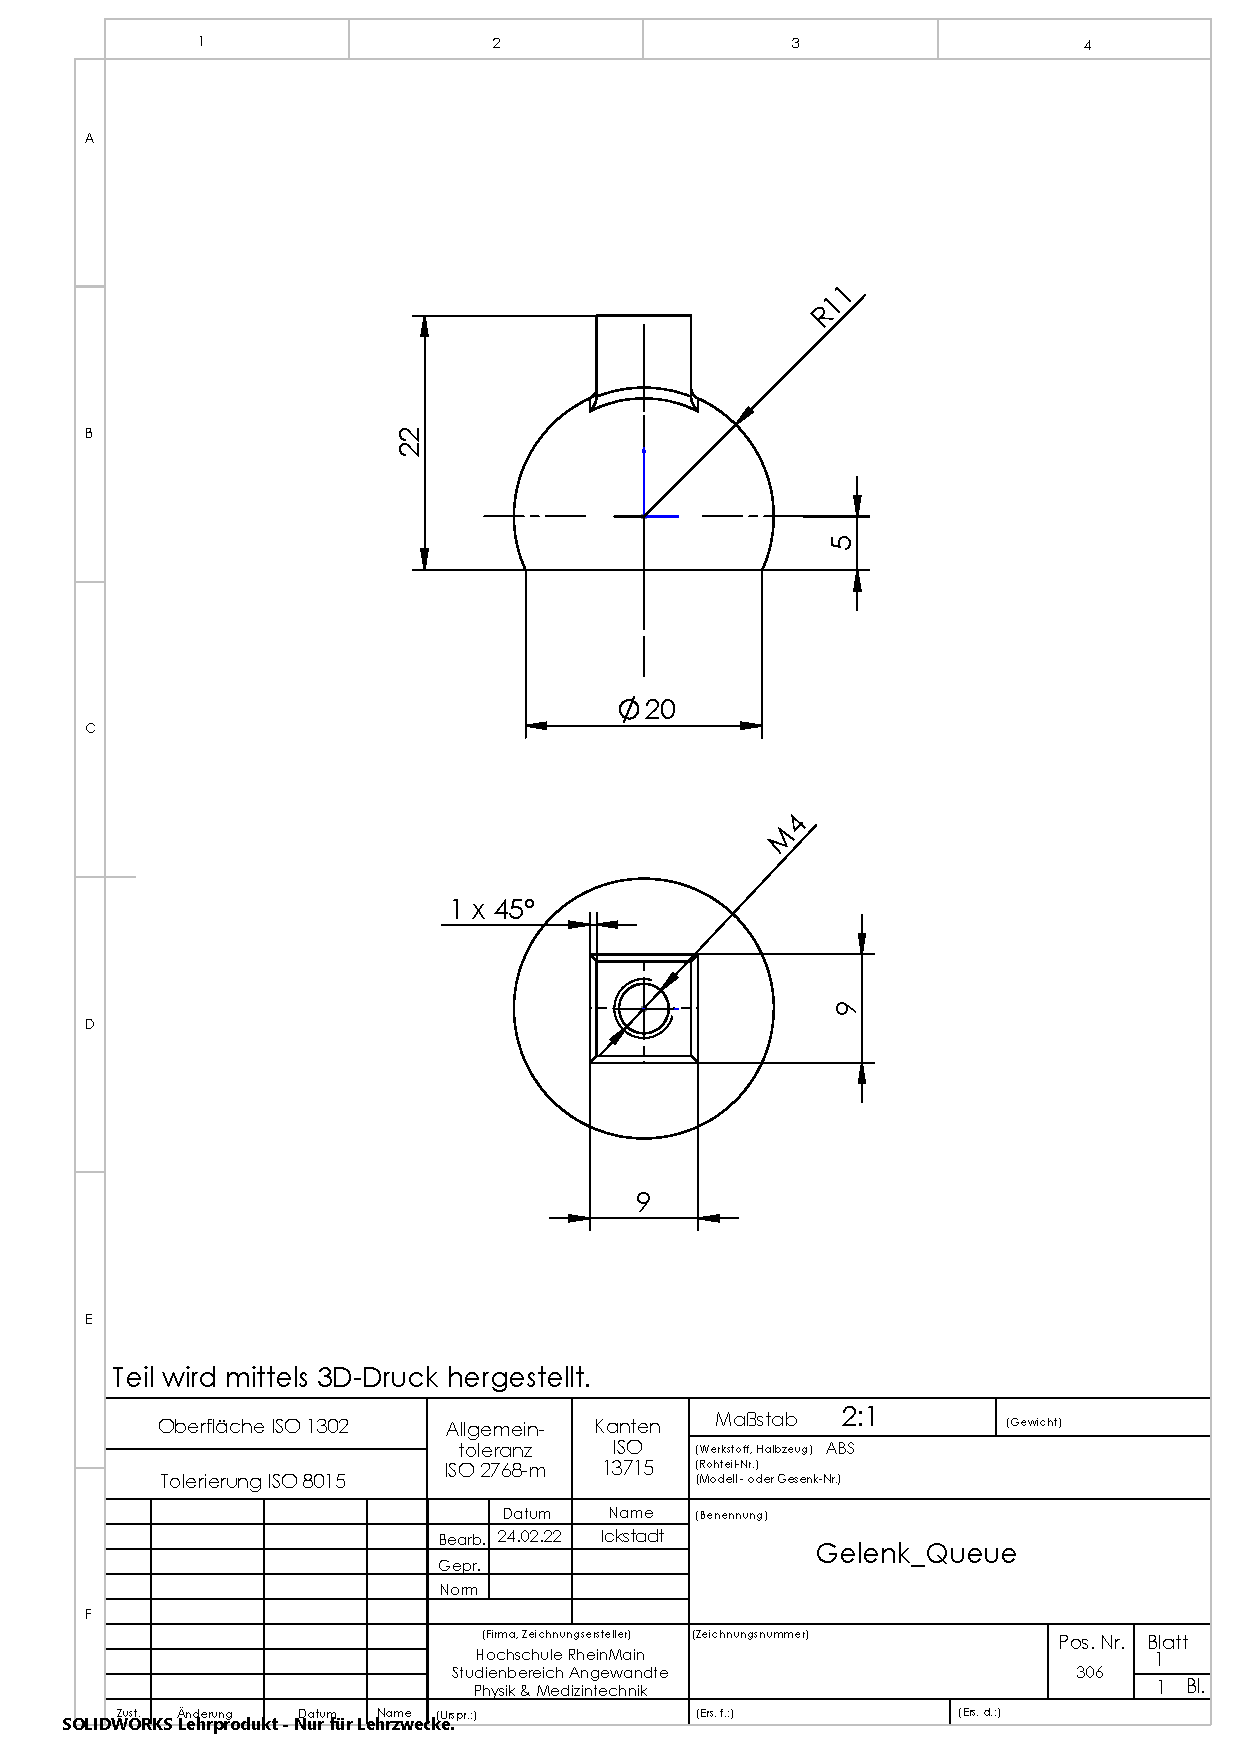
\includepdf[pages=-, angle=0, pagecommand={\thispagestyle{plain}}]{Abb/CAD/Drawings/Gelenk-Queue.pdf}
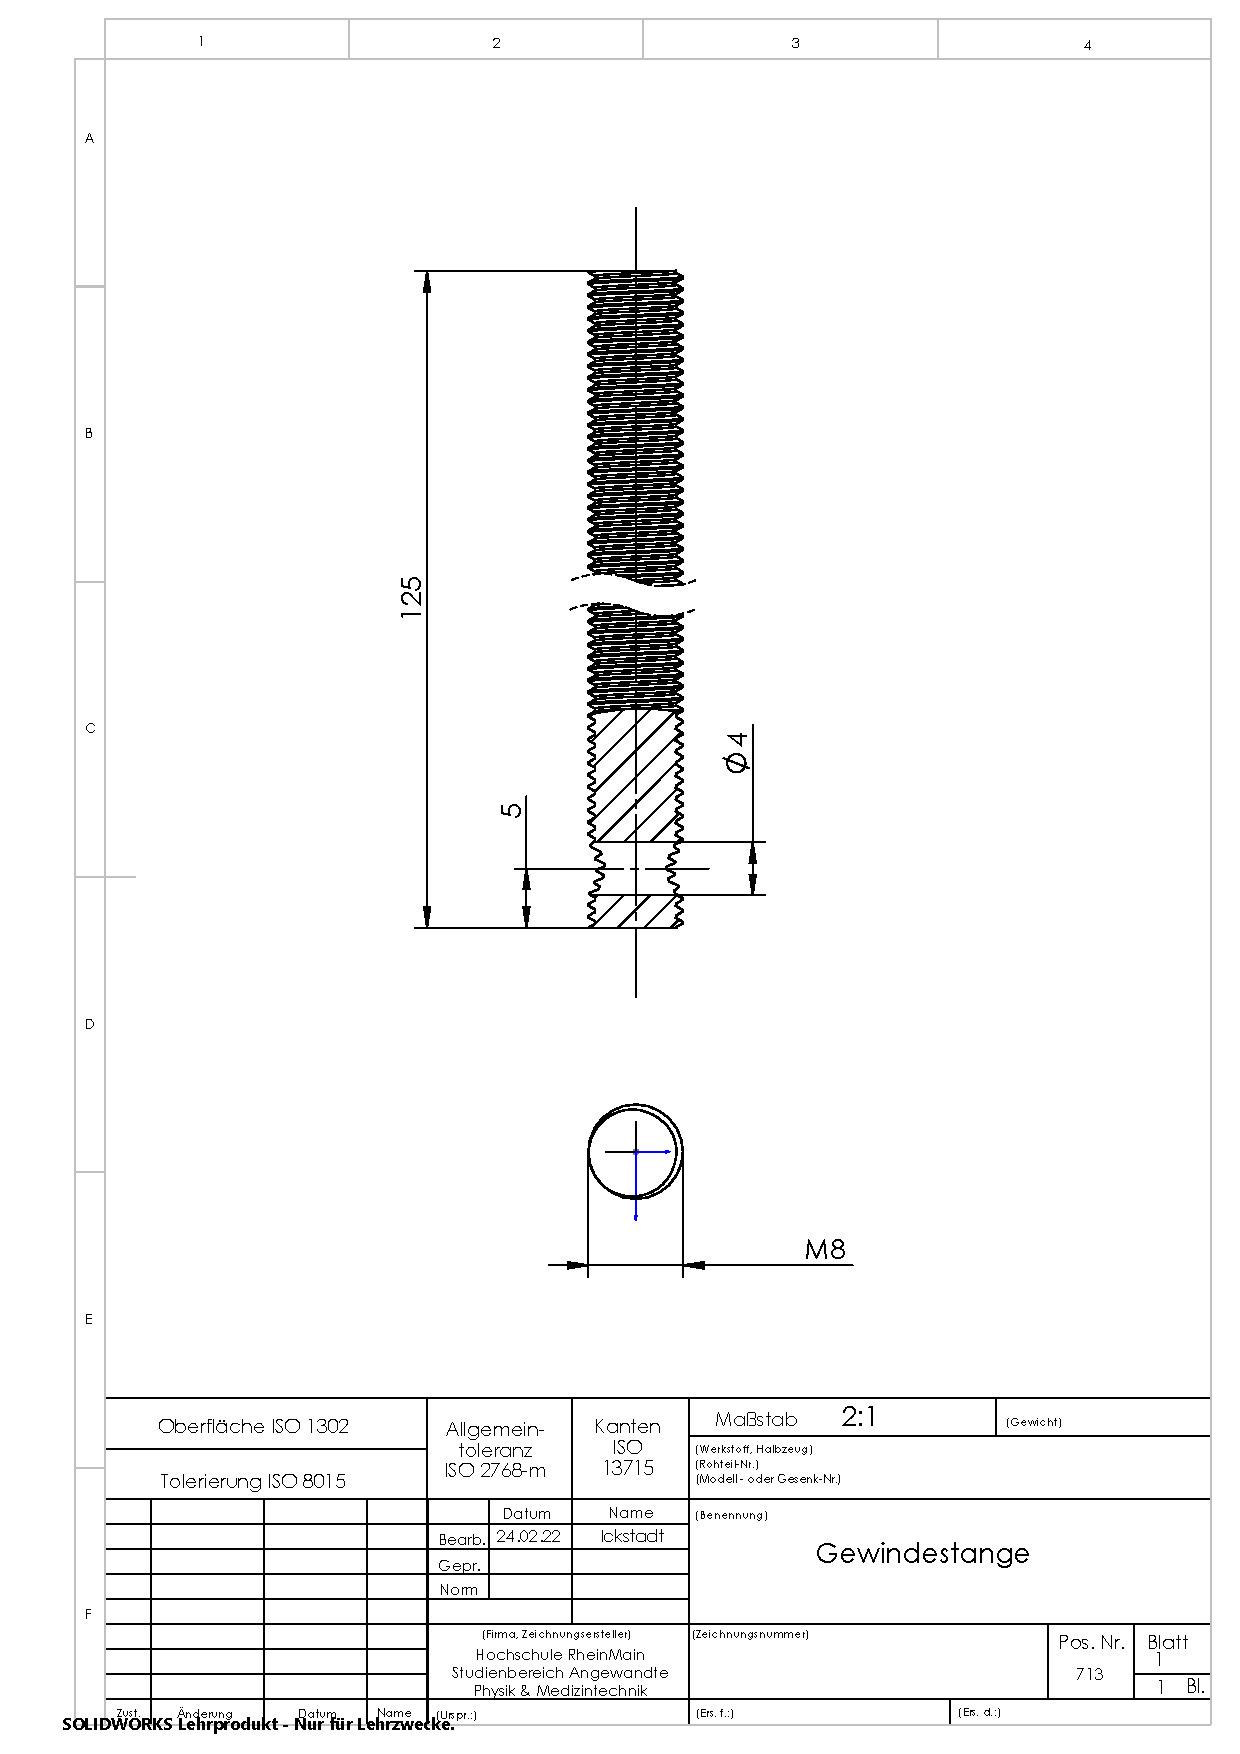
\includepdf[pages=-, angle=0, pagecommand={\thispagestyle{plain}}]{Abb/CAD/Drawings/Gewindestange.pdf}
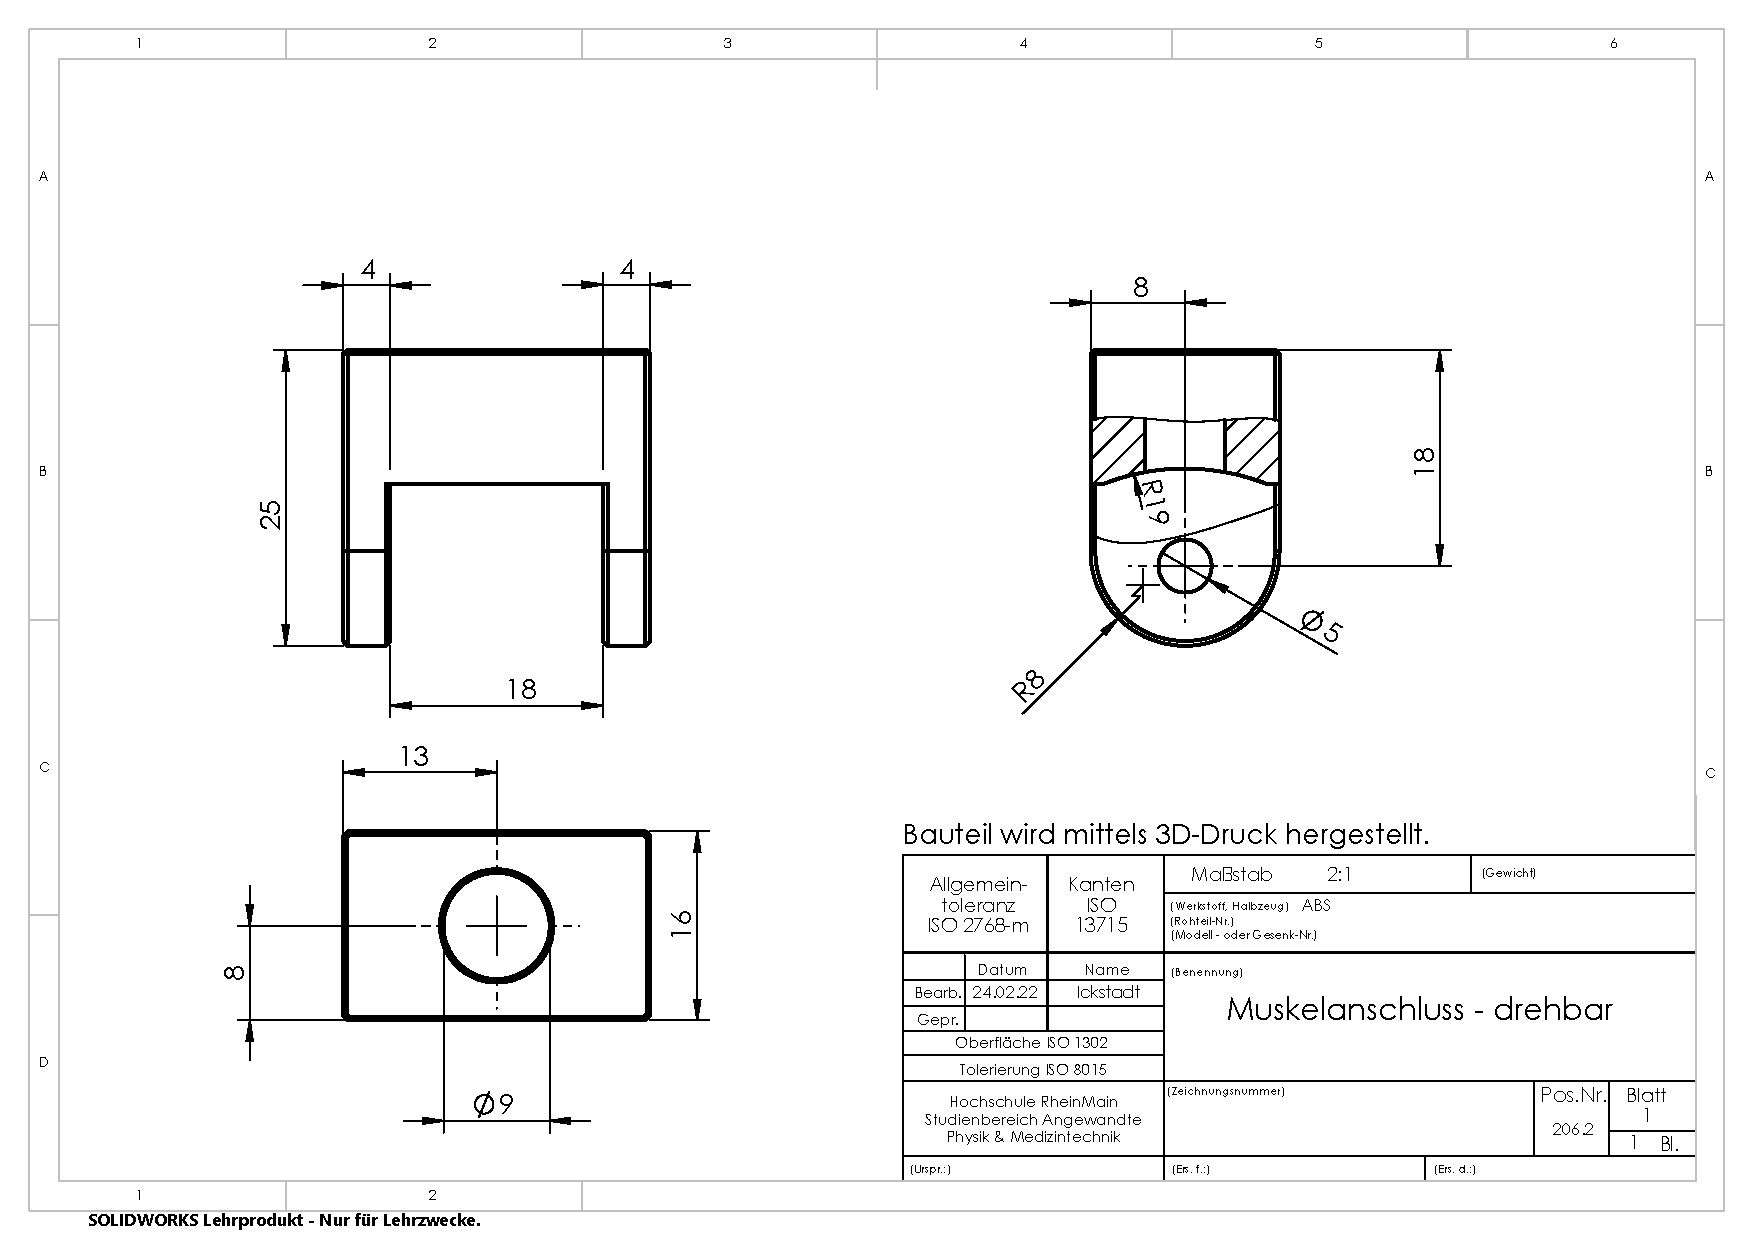
\includepdf[pages=-, angle=90, pagecommand={\thispagestyle{plain}}]{Abb/CAD/Drawings/Muskelanschluss-drehbar.pdf}
%
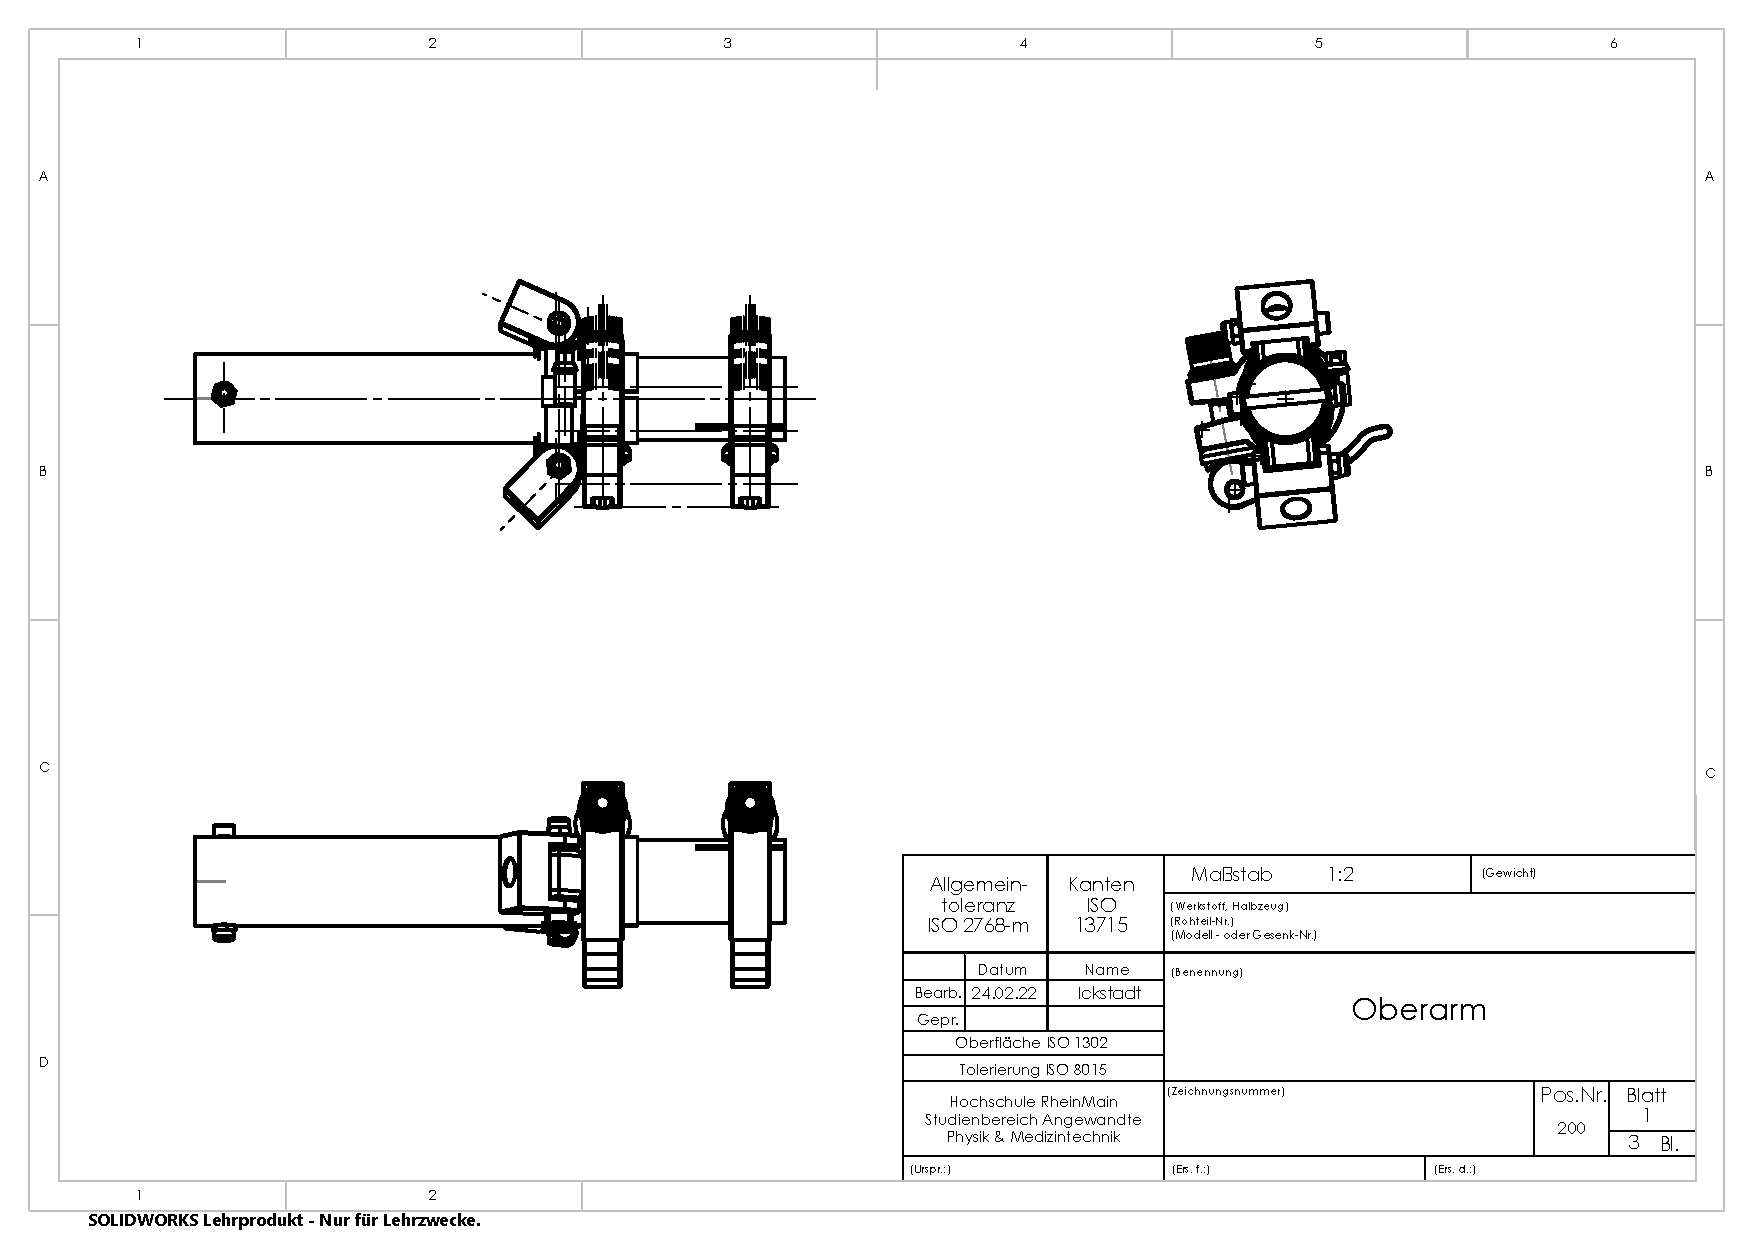
\includepdf[pages=1-2, angle=90, pagecommand={\thispagestyle{plain}}]{Abb/CAD/Drawings/Oberarm.pdf}
\includepdf[pages=3, angle=0, pagecommand={\thispagestyle{plain}}]{Abb/CAD/Drawings/Oberarm.pdf}
%
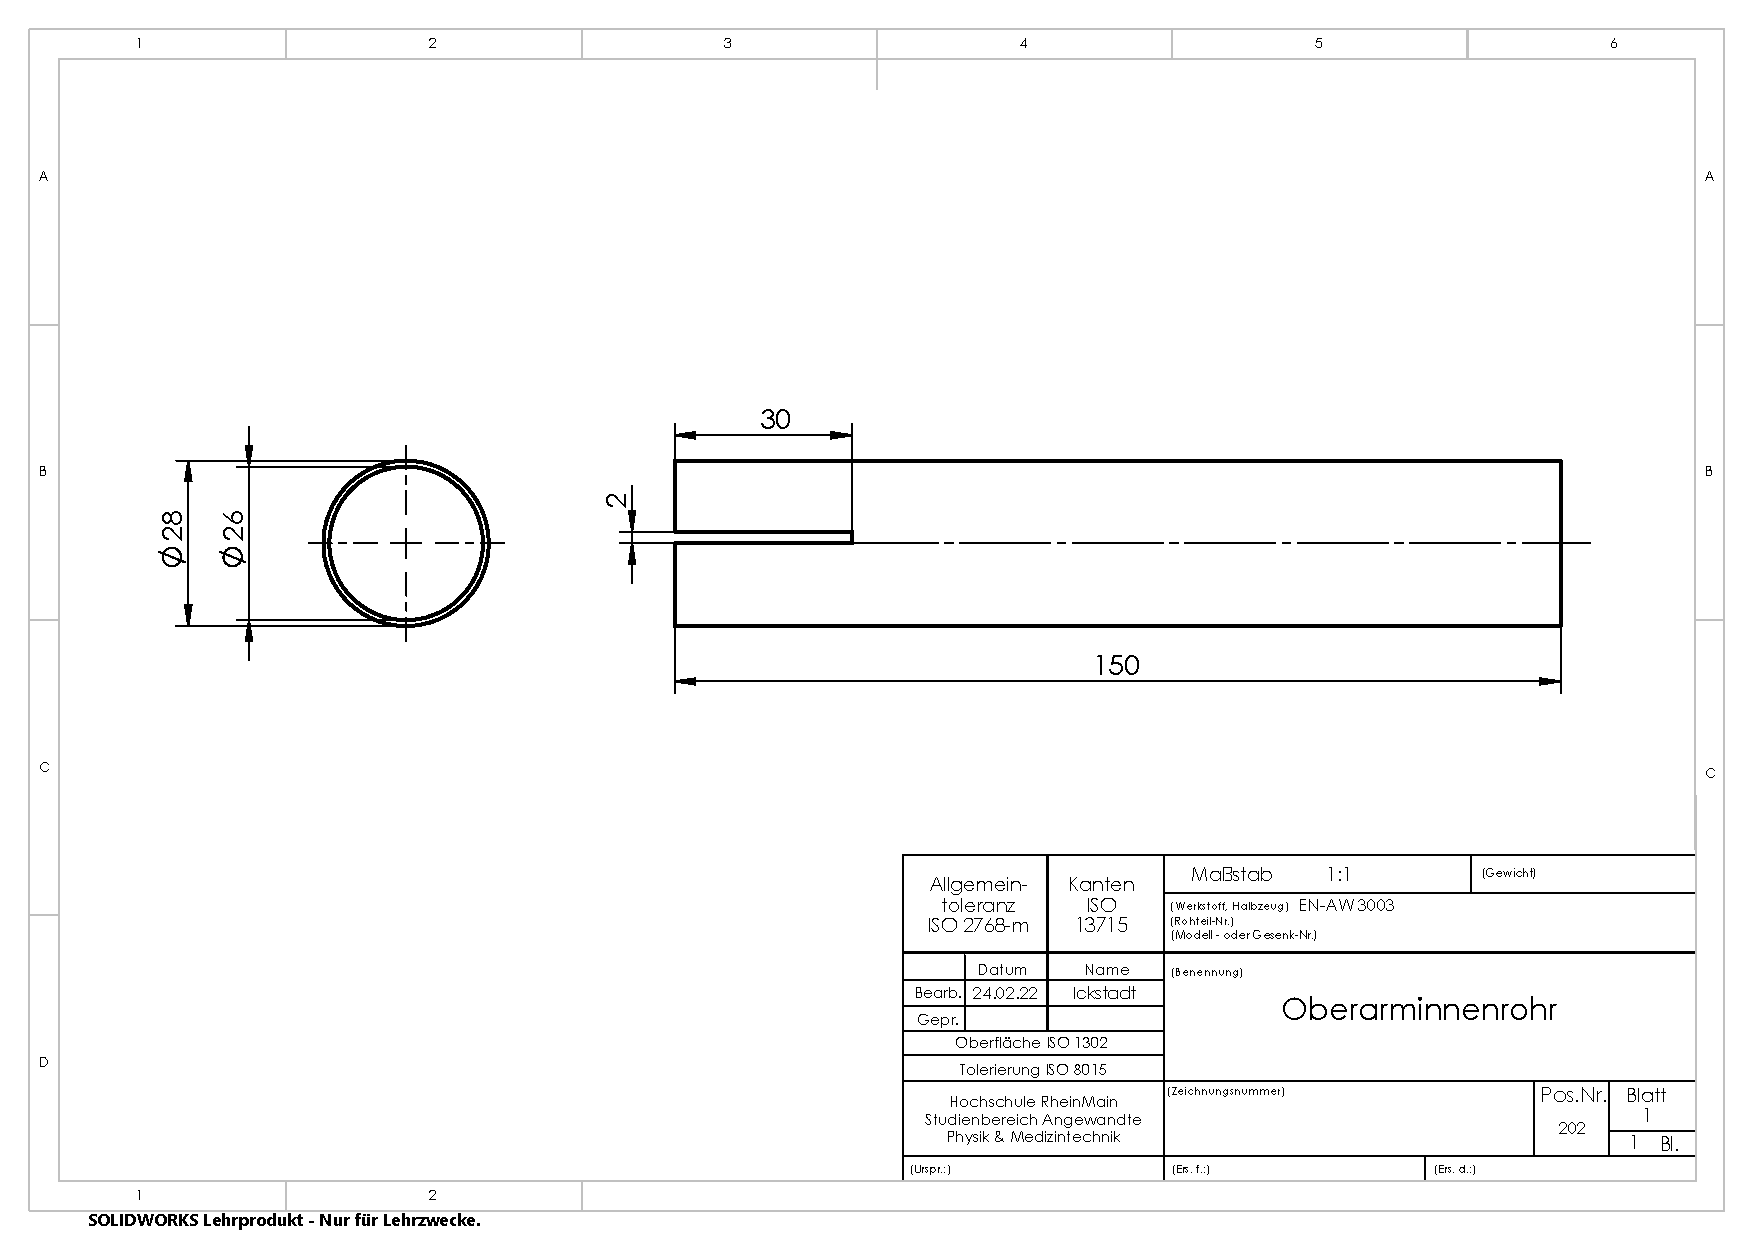
\includepdf[pages=-, angle=90, pagecommand={\thispagestyle{plain}}]{Abb/CAD/Drawings/Oberarminnenrohr.pdf}
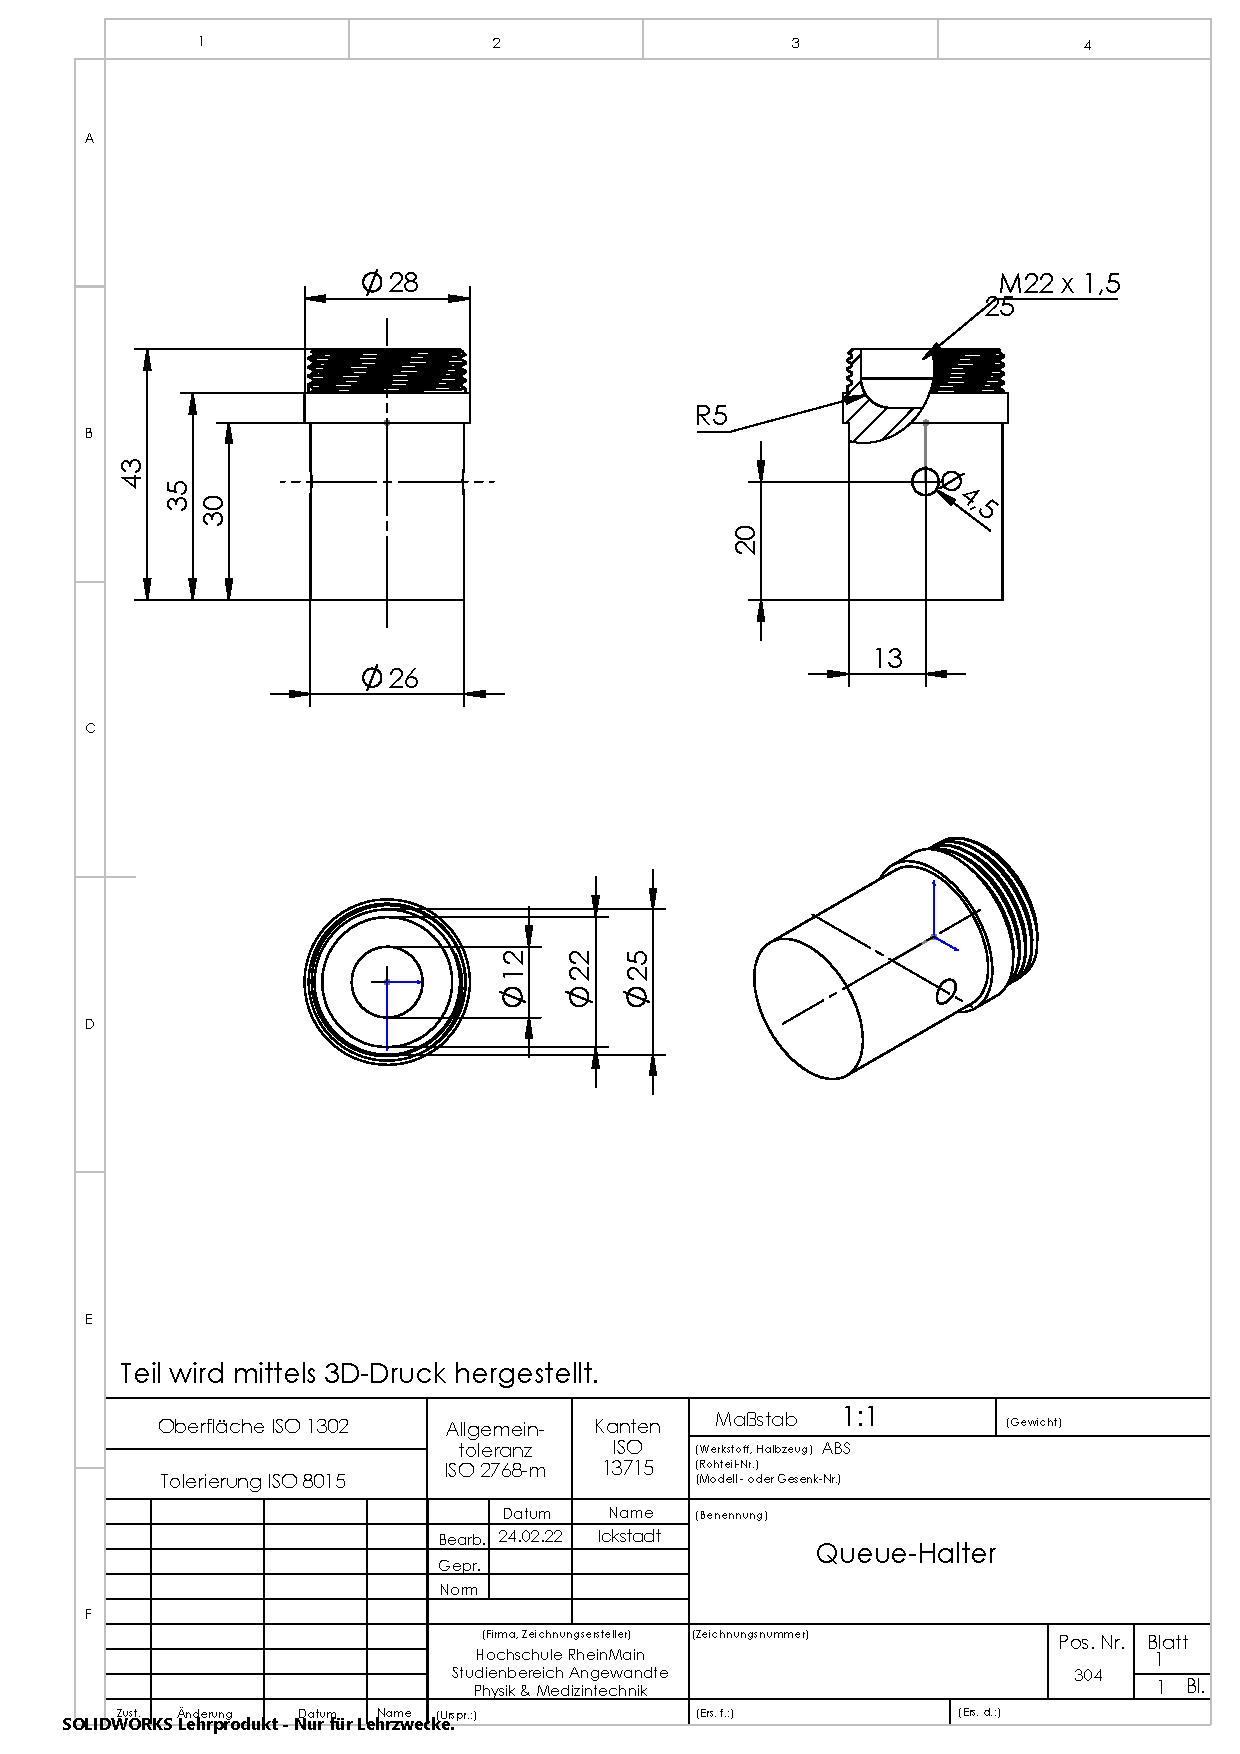
\includepdf[pages=-, angle=0, pagecommand={\thispagestyle{plain}}]{Abb/CAD/Drawings/Queue-Halter.pdf}
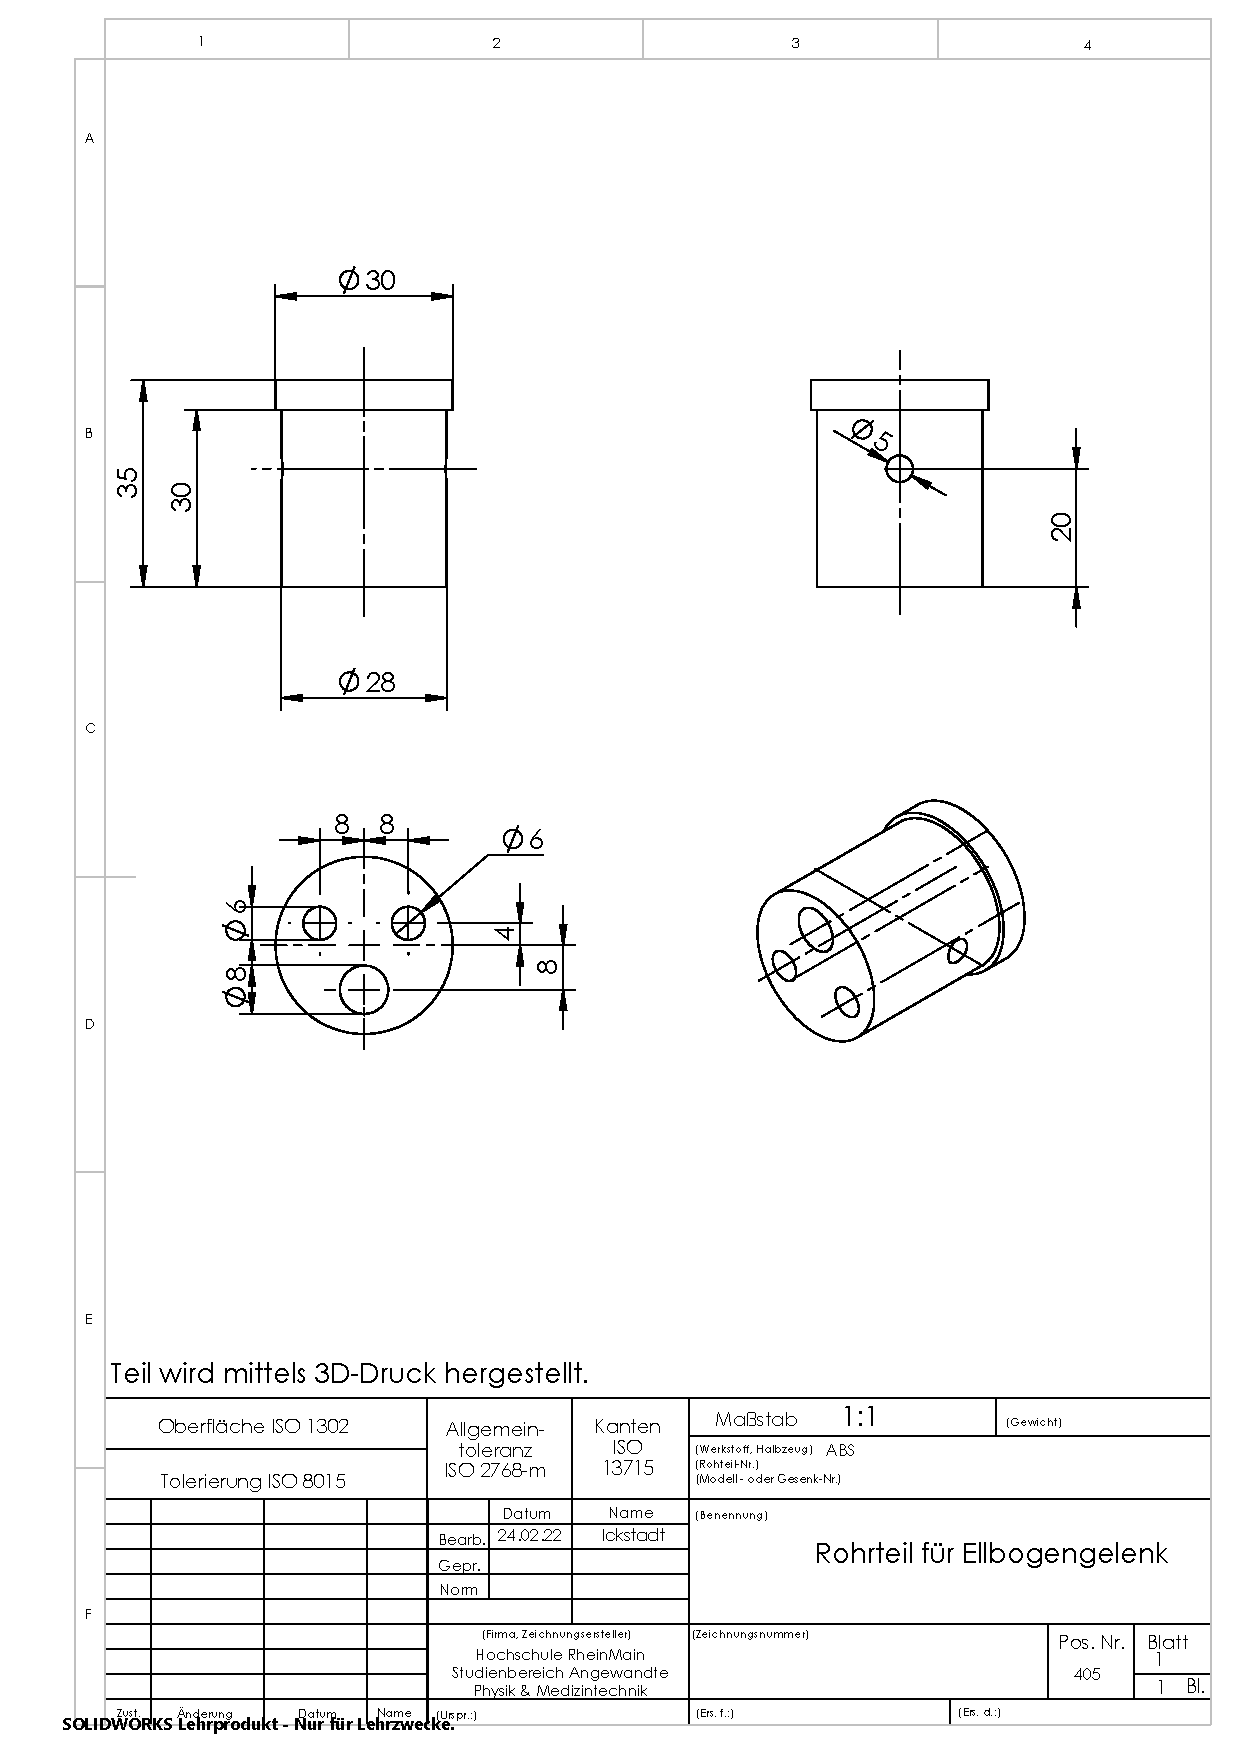
\includepdf[pages=-, angle=0, pagecommand={\thispagestyle{plain}}]{Abb/CAD/Drawings/Rohrteil-fuer-Ellbogengelenk.pdf}
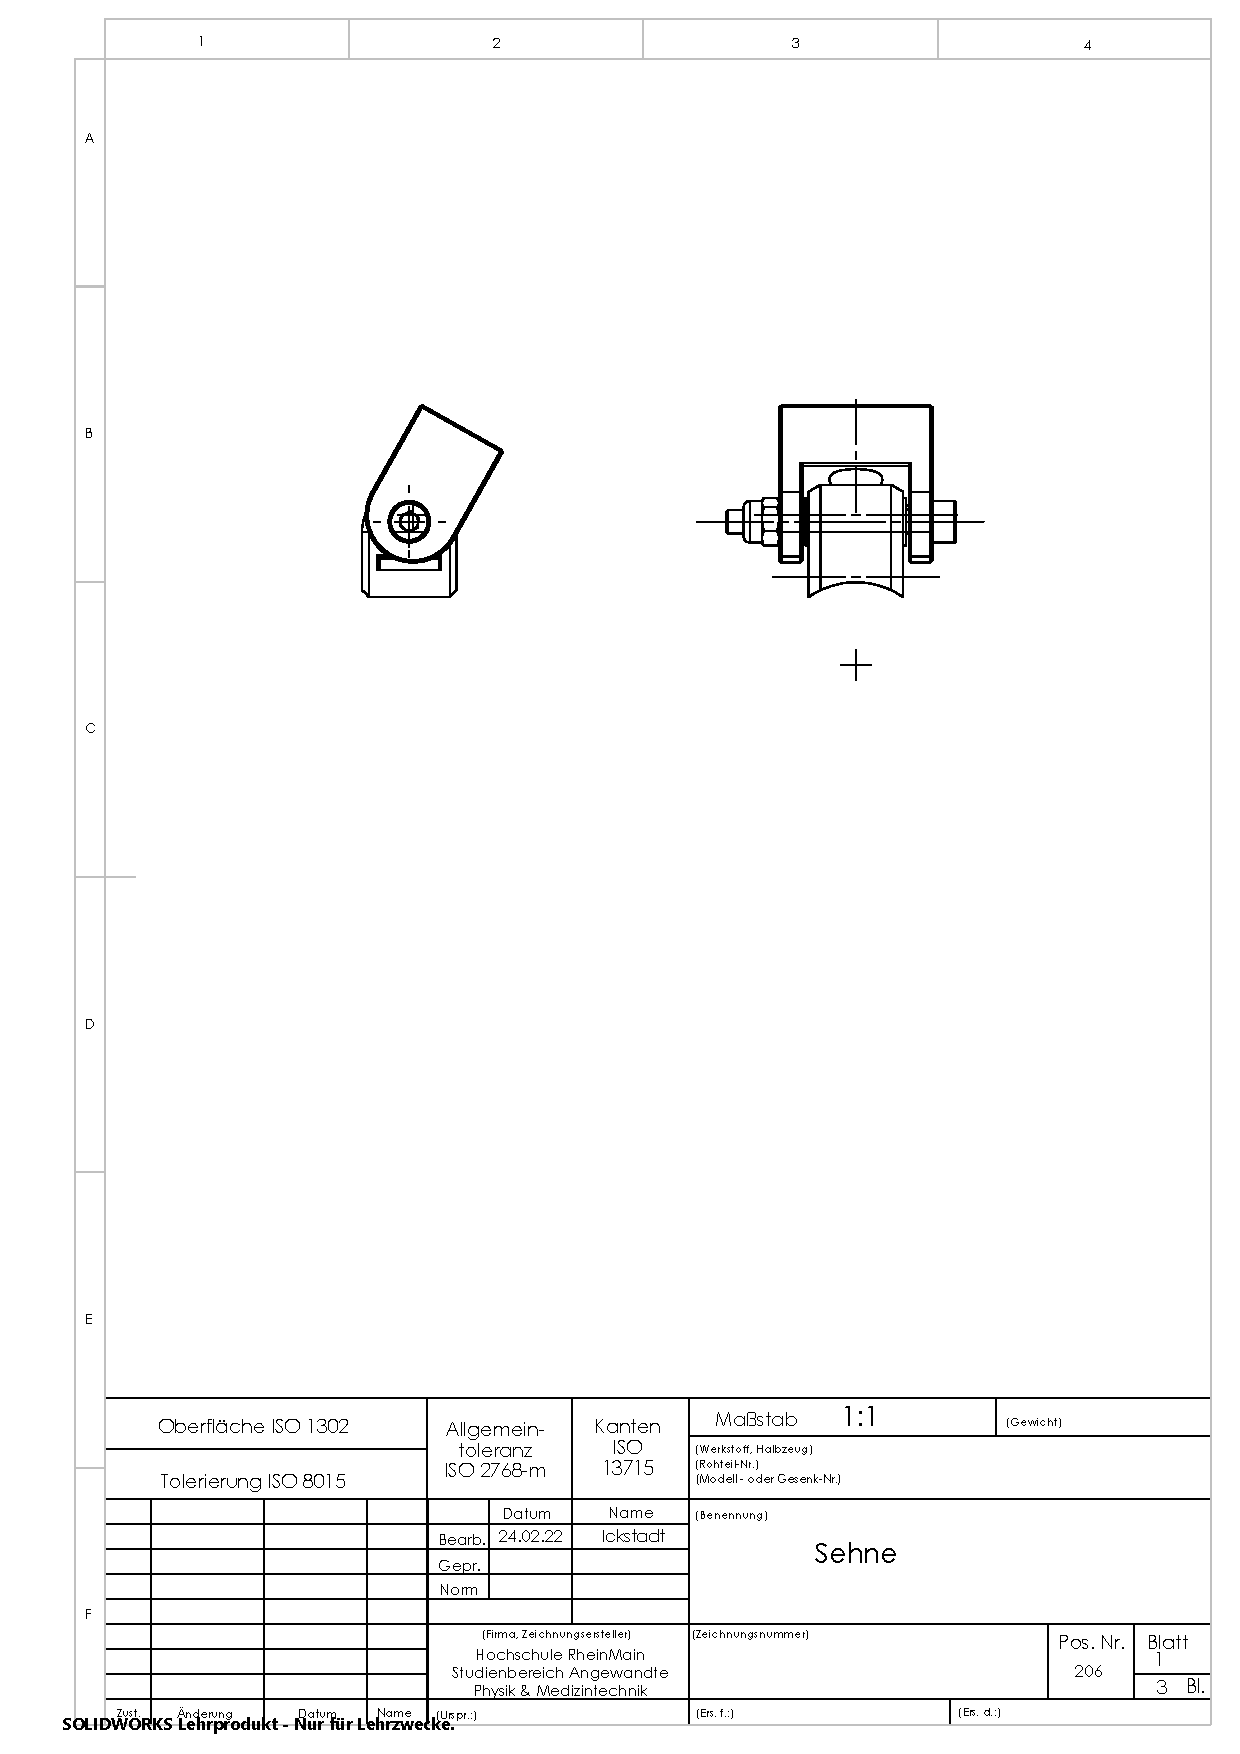
\includepdf[pages=-, angle=0, pagecommand={\thispagestyle{plain}}]{Abb/CAD/Drawings/Sehne.pdf}
%
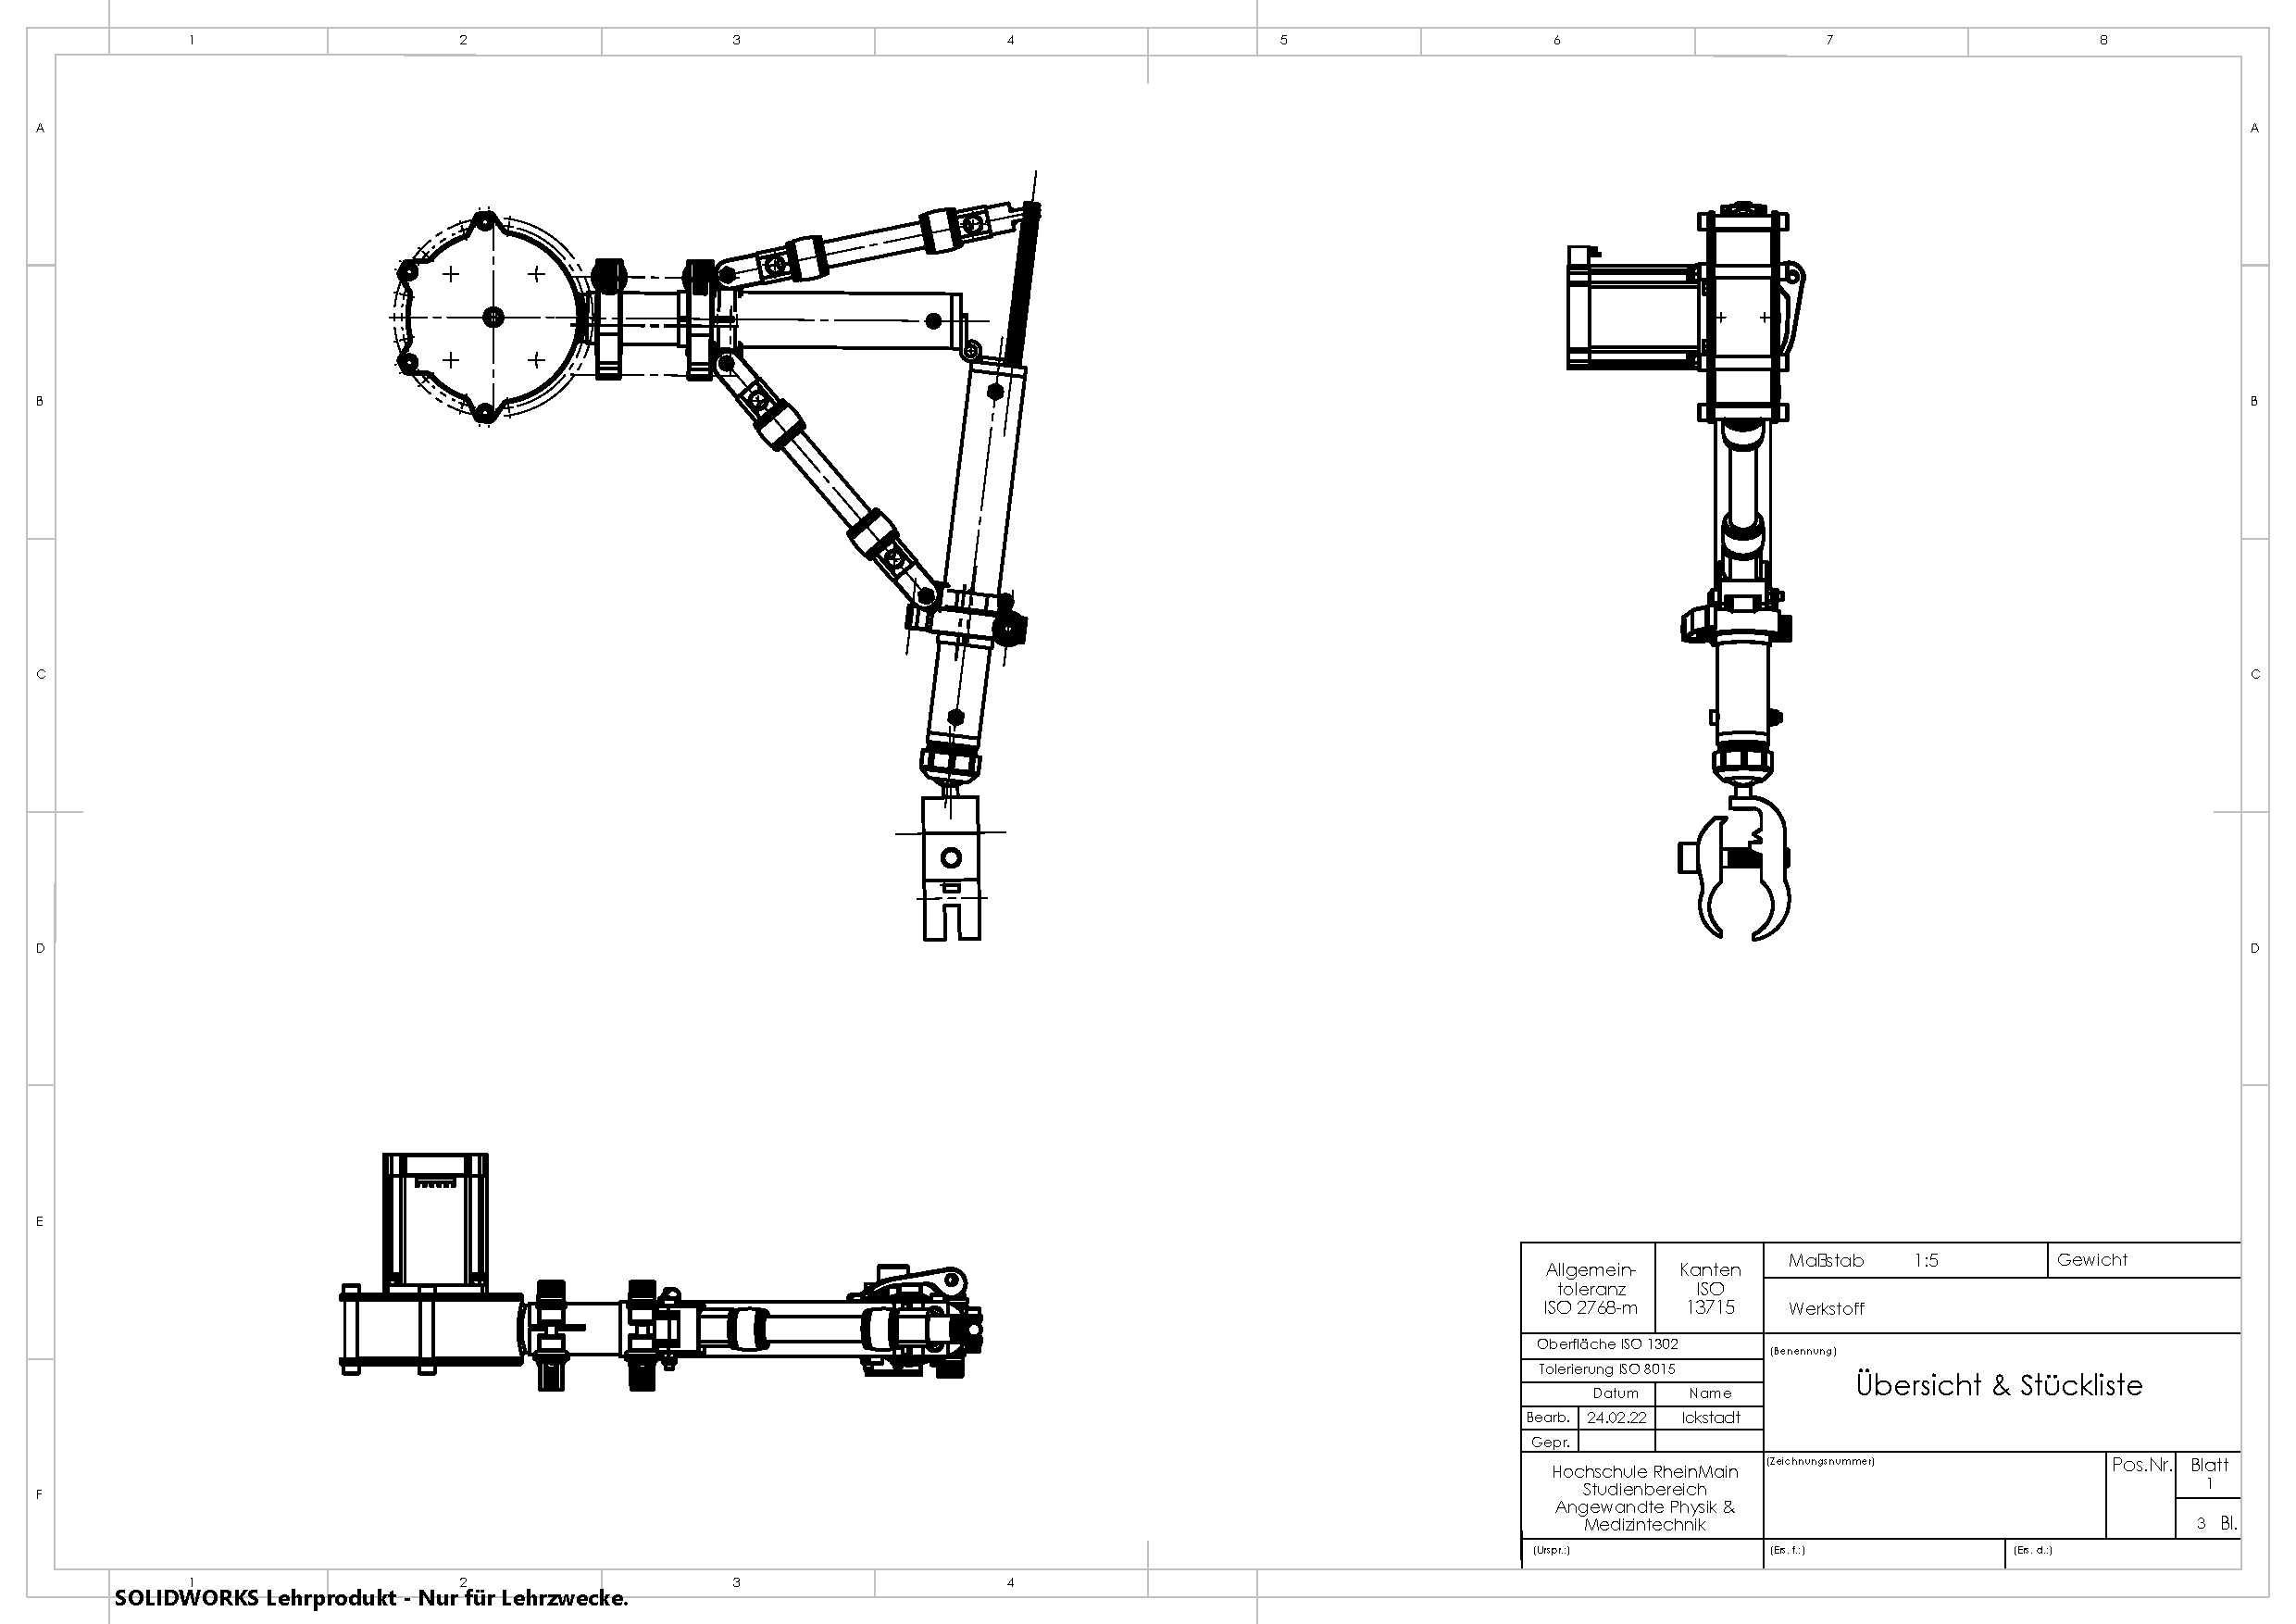
\includepdf[pages=1, angle=90, pagecommand={\thispagestyle{plain}}]{Abb/CAD/Drawings/Uebersicht-und-Stueckliste.pdf}
\includepdf[pages=2, angle=90, pagecommand={\thispagestyle{plain}}]{Abb/CAD/Drawings/Uebersicht-und-Stueckliste.pdf}
%
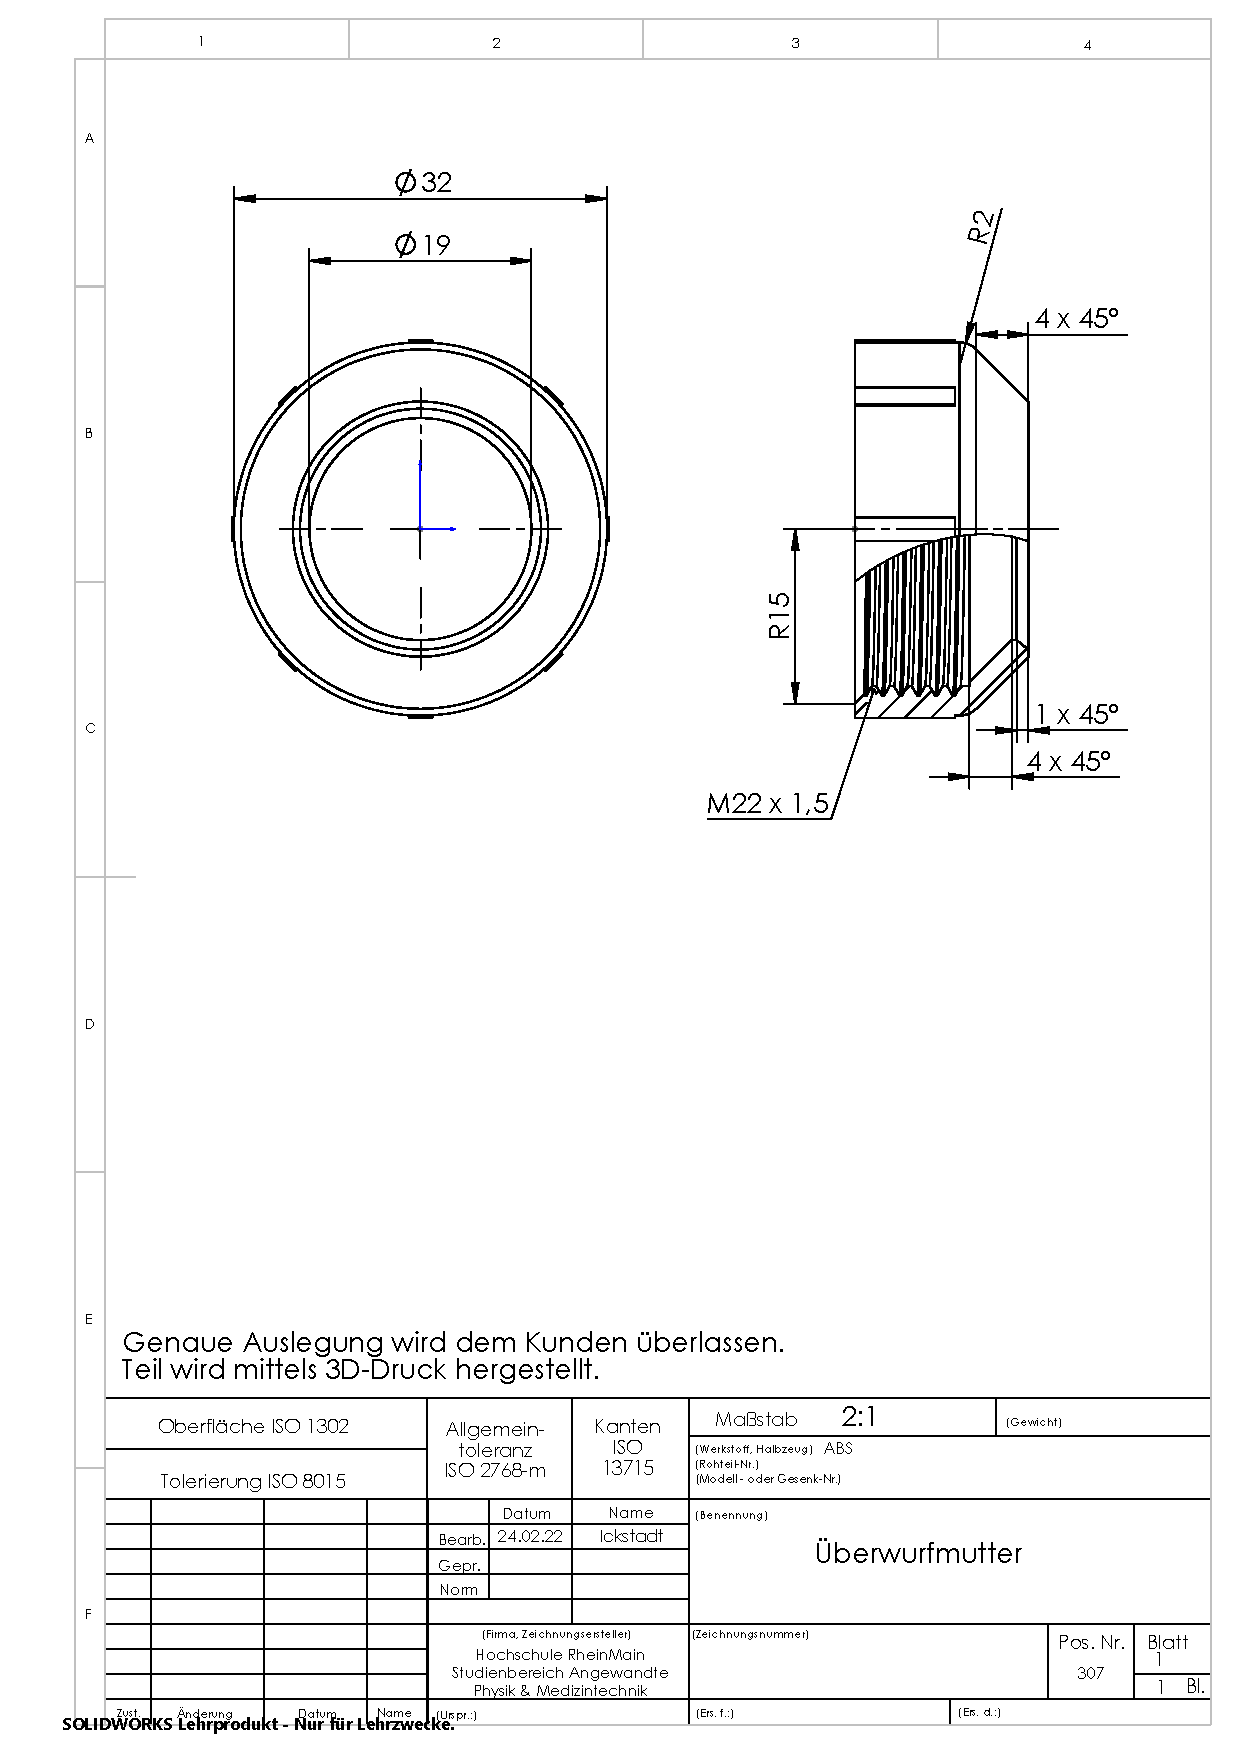
\includepdf[pages=-, angle=0, pagecommand={\thispagestyle{plain}}]{Abb/CAD/Drawings/Ueberwurfmutter.pdf}
%
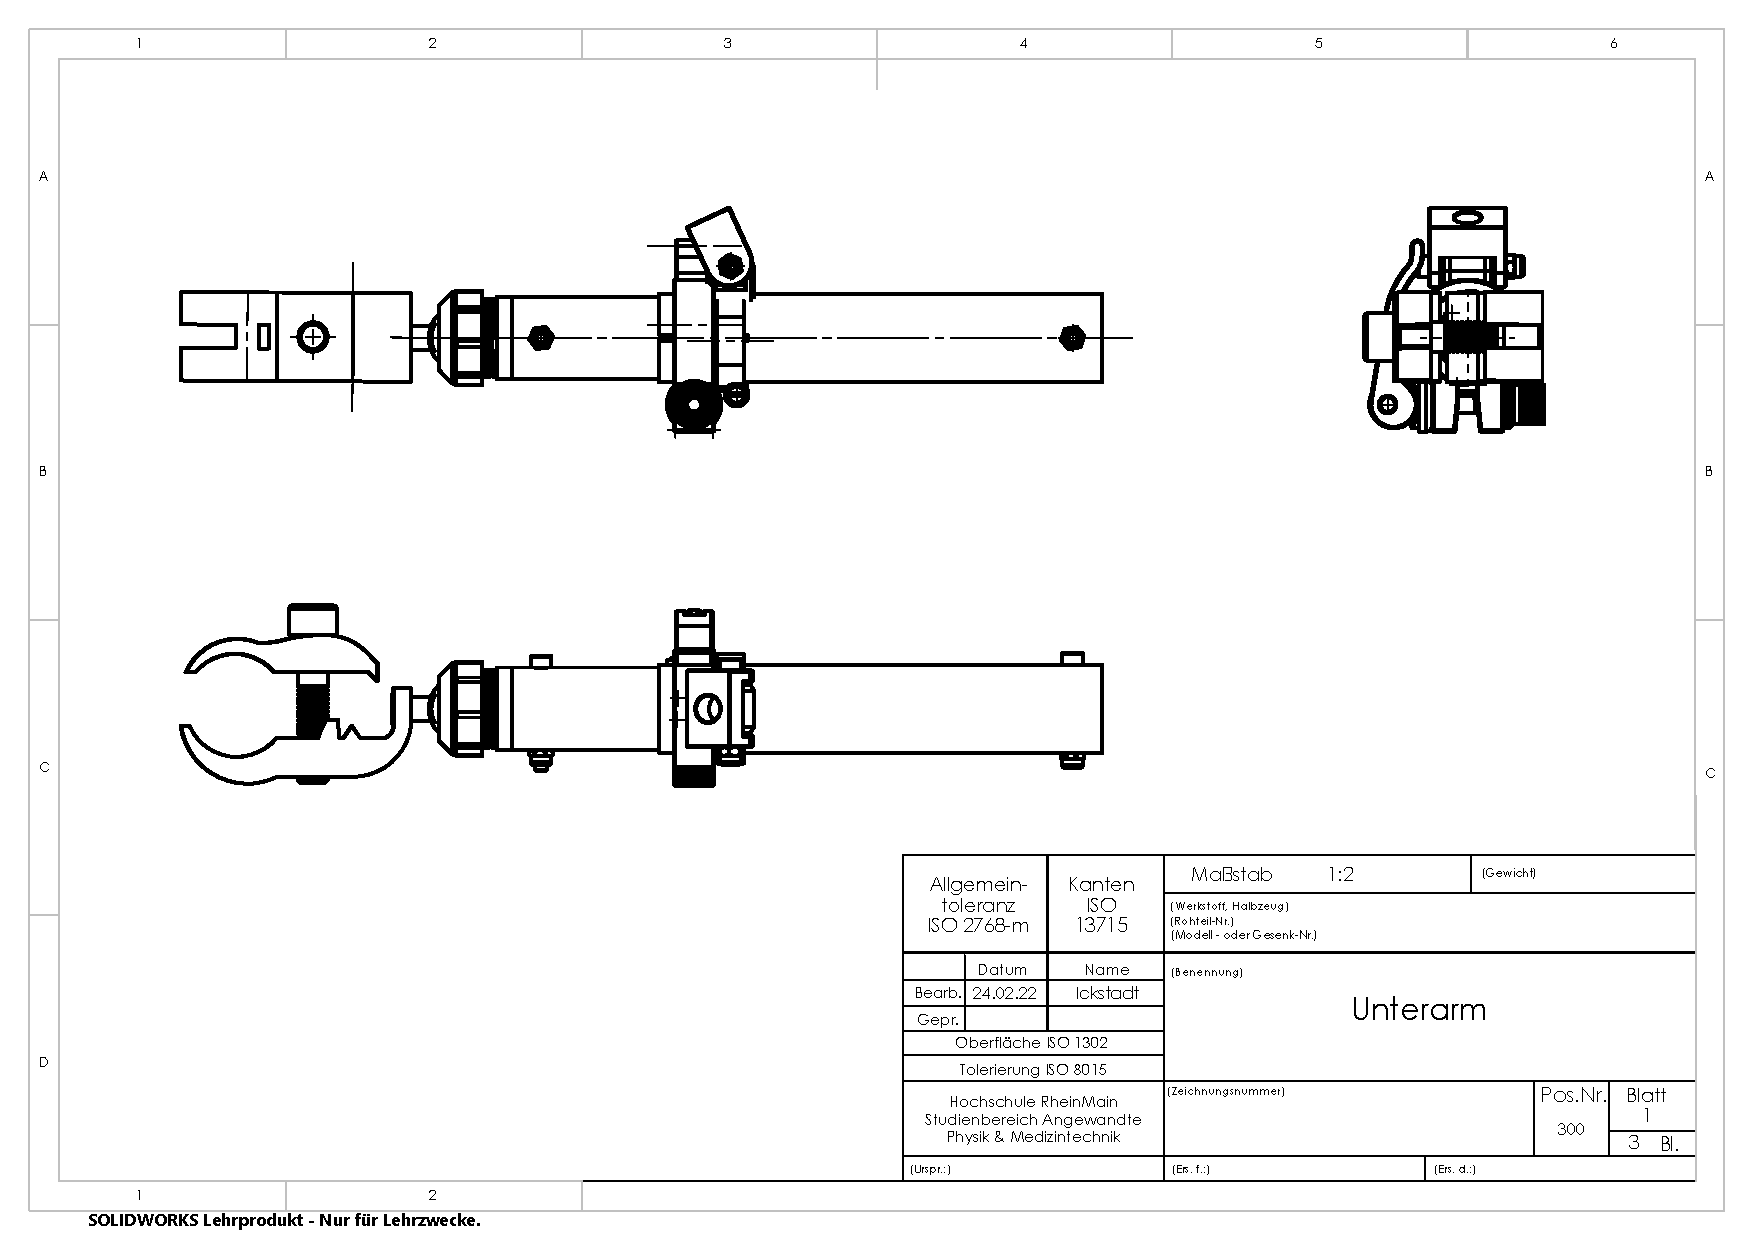
\includepdf[pages=1-2, angle=90, pagecommand={\thispagestyle{plain}}]{Abb/CAD/Drawings/Unterarm.pdf}
\includepdf[pages=3, angle=0, pagecommand={\thispagestyle{plain}}]{Abb/CAD/Drawings/Unterarm.pdf}
%
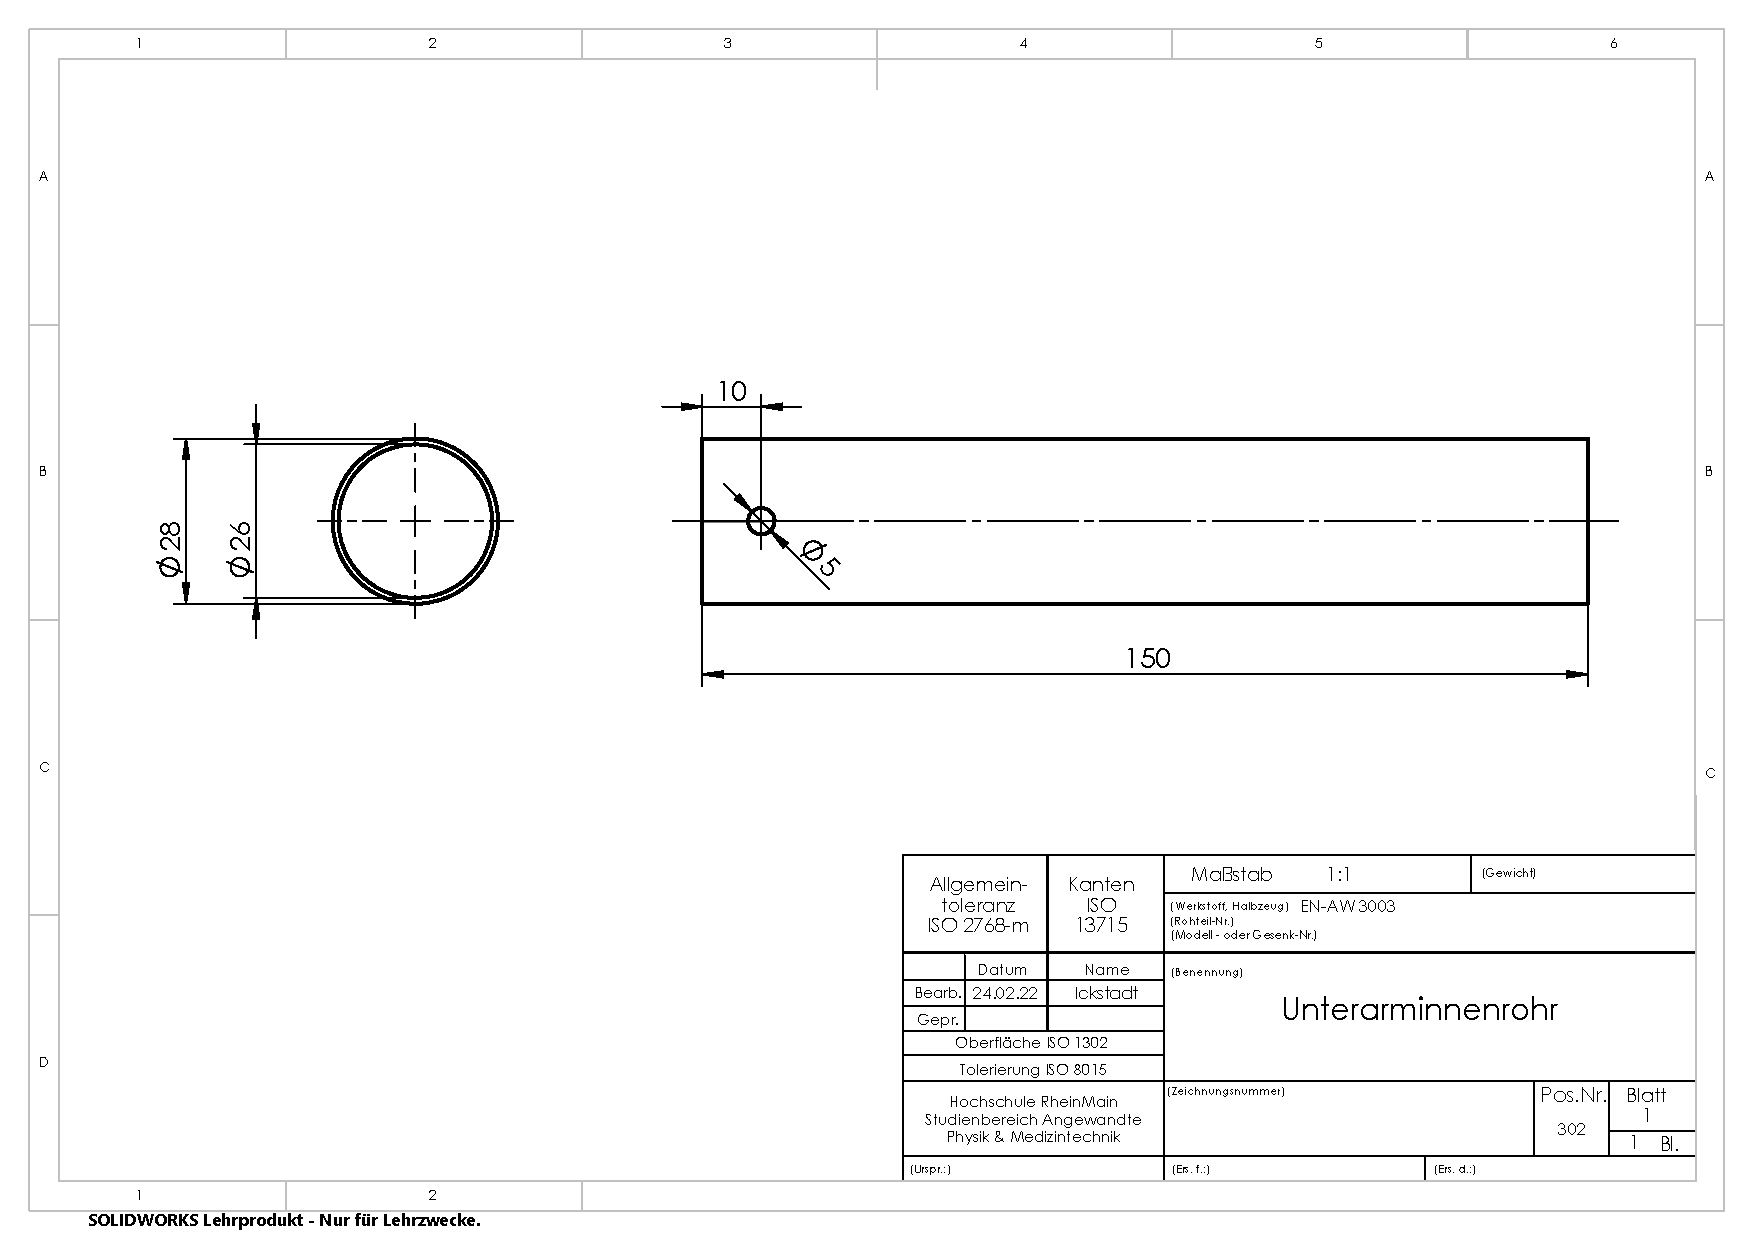
\includepdf[pages=-, angle=90, pagecommand={\thispagestyle{plain}}]{Abb/CAD/Drawings/Unterarminnenrohr.pdf}
% \includepdf[pages=-, angle=0, pagecommand={\thispagestyle{plain}}]{Abb/CAD/Drawings/.pdf}
\setlength{\voffset}{-2.5 cm}
\setlength{\hoffset}{-2 cm}